
\documentclass[12pt,a4paper,twoside]{book}

%% general usepackage stuff
\usepackage{times}
\usepackage{mathptmx}
\usepackage{booktabs}
\usepackage{graphicx}
\usepackage{titlesec}
\usepackage{amssymb}

\usepackage{color}

%% labels and page stuff
\renewcommand{\labelitemi}{$\diamond$}
\renewcommand{\labelitemii}{$\circ$}

\setcounter{tocdepth}{4} %% TODO: remove later again
\setcounter{secnumdepth}{3}

%\setlength{\oddsidemargin}{-0.5cm}
%\setlength{\evensidemargin}{-0.5cm}

\setlength{\oddsidemargin}{4.58mm}%final
\setlength{\evensidemargin}{-4.92mm}%final


\setlength{\textwidth}{15.95cm}%final
\setlength{\textheight}{23.5cm}
\setlength{\voffset}{-1.45cm} %


%% todo
\newcommand{\todo}[1]{\textcolor{red}{[todo: }#1\textcolor{red}{]}}
\newcommand{\todoh}[1]{} 
\newcommand{\done}[1]{} 

%% smallerText
\newcommand{\smallerTextSize}{10}
\newcommand{\smallerTextSkip}{12}
\newcommand{\smallerBegin}{\fontsize{\smallerTextSize}{\smallerTextSkip}\selectfont}
\newcommand{\smallerEnd}{\normalsize}
\newcommand{\smaller}[1]{\smallerBegin #1\smallerEnd}

%%reference to defintion
\newcommand{\defref}[1]{\ref{#1} on page \pageref{#1}}

%% special, short for shell
\newcommand{\shl}[1]{\sf \small #1\rm\normalsize}

%% indentation in tables
\newcommand{\tabind}[1]{\rule{#1mm}{0cm}}

%% smaller in captions
\newcommand{\captionfonts}{\smallerBegin}
                                                                                                                                                                              
\makeatletter  % Allow the use of @ in command names
\long\def\@makecaption#1#2{%
  \vskip\abovecaptionskip
  \sbox\@tempboxa{{\captionfonts #1: #2}}%
  \ifdim \wd\@tempboxa >\hsize
    {\captionfonts #1: #2\par}
  \else
    \hbox to\hsize{\hfil\box\@tempboxa\hfil}%
  \fi
  \vskip\belowcaptionskip}
\makeatother   % Cancel the effect of \makeatletter

%% clear page before new chapter
\makeatletter
\def\cleardoublepage{\clearpage\if@twoside \ifodd\c@page\else
\hbox{}
\vspace*{\fill}
\begin{center}
%This page intentionally contains only this sentence.
\end{center}
\vspace{\fill}
\thispagestyle{empty}
\newpage
\if@twocolumn\hbox{}\newpage\fi\fi\fi}
\makeatother

%% abbreviations
\usepackage{nomencl}
\let\abbrev\nomenclature
\renewcommand{\nomname}{List of Abbreviations}
\setlength{\nomlabelwidth}{.25\hsize}
\renewcommand{\nomlabel}[1]{#1 \dotfill}
\setlength{\nomitemsep}{-\parsep}
\makenomenclature
\newcommand{\Listofabbrev}{
\printnomenclature
\newpage
}

%% chapter title formatting
\titleformat{\chapter}[display]{ \raggedleft }{\fontsize{52}{63}\selectfont \bf \thechapter }{0.2cm}{\fontsize{32}{38.7}\selectfont  }[]

%% haeder formatting
\renewcommand{\chaptermark}[1]{%
\markboth{\chaptername
\ \thechapter.\ #1}{}}
\renewcommand{\sectionmark}[1]{\markright{\thesection.\ #1}}
\usepackage{fancyhdr}
\pagestyle{fancy}
\fancyhf[LEH,ROH]{\thepage}
\fancyhf[REH]{\smaller{\nouppercase{\leftmark}}}
\fancyhf[LOH]{\smaller{\it \nouppercase{\rightmark}}}
\fancyhf[COF]{\rule{0.2cm}{0.0cm}}
\fancyhf[CEF]{\rule{0.2cm}{0.0cm}}
\renewcommand{\headrulewidth}{0pt}

%% macro for figures
%\usepackage{svg}
%\usepackage{amsmath}
%\newcommand{\printlabel}{}
%\newcommand{\abcdef}[1]{\tiny #1 \normalsize}

		%% arguments: graphics file, label, caption, smallcaption
\newcommand{\insertFigure}[4]{\begin{figure}[top] \smallerBegin \centering \includegraphics{#1}  \\  \caption{\label{#2}\smallerBegin #3 \footnotesize{#4}  \smallerEnd }  
\end{figure}	}
%% macro for figures with short caption
		%% arguments: graphics file, label, caption, smallcaption, shortcaption
\newcommand{\insertFigureShort}[5]{\begin{figure}[top] \smallerBegin \centering \includegraphics{#1} \label{#2} \\ \caption[#5]{\smallerBegin #3 \footnotesize{#4} \smallerEnd } 
\end{figure}	}
%\renewcommand{\topfraction}{1}

\newcommand{\spaceafterpar}{\vspace{14.48pt}}

\renewcommand{\floatpagefraction}{.75} % vorher: .5
\renewcommand{\textfraction}{.1}       % vorher: .2
\renewcommand{\topfraction}{.8}        % vorher: .7
\renewcommand{\bottomfraction}{.5} 
\setcounter{topnumber}{3}              % vorher: 2
\setcounter{bottomnumber}{2}           % vorher: 1
\setcounter{totalnumber}{5}            % vorher: 3
%from: http://www.matthiaspospiech.de/latex/vorlagen/allgemein/preambel/9/

%macros for tables
    %% arguments: columns
\newcommand{\tableBegin}[1]{\begin{table}[top] \begin{center} \smallerBegin \begin{tabular}{#1}}
		%% arguemtns: caption, label
\newcommand{\tableEnd}[2]{ \end{tabular} \smallerEnd \end{center} \caption{#1} \label{#2}	\end{table}}

%% shortcuts
\newcommand{\emit}[1]{\item \emph{#1}:}
\newcommand{\firstappear}[2]{\emph{#1} (#2) \abbrev{#2}{#1}}

\hyphenation{or-gan-izing}

%% definitions

\newtheorem{definition}{Definition}

%% examples
\newcommand{\exampleBeginText}[1]{\paragraph{#1}}
\newcommand{\exampleEnd}{\vspace{6mm}}
\newcommand{\exampleBegin}{\exampleBeginText{Example}}

%algorithms
\usepackage[english,ruled,vlined, slide, norelsize]{algorithm2e}

%placements
\usepackage{float}

%references
\usepackage[numbers,sort]{natbib}
\setlength{\bibsep}{0.0pt}
\bibliographystyle{plainnat}

%ref imgs
\usepackage{hyperref}
\usepackage{cleveref}
\usepackage{todonotes}
\usepackage[onehalfspacing]{setspace}

\usepackage{csvsimple}


% Front Matter
\singlespacing
\newcommand{\titleLineOne}{Graph-based Recommendation of Optimized IT-Service Deployment Scripts based on crowdsourced Data}
\newcommand{\titleLineTwo}{}
\newcommand{\titleLineThree}{}
\newcommand{\documentdate}{\today}
\newcommand{\studentname}{Lars Lange}
\newcommand{\abstracttextde}{Infrastructure as Code hat in den letzten Jahren durch die DevOps-Bewegung viel an Bedeutung gewonnen, aber bisher hat noch niemand ein Empfehlungssystem für Deployment-Skripte entwickelt, das basierend auf benutzerdefinierten Eingaben ähnliche Skripte vorschlägt, die durch einen vorberechneten Wert ermittelt werden. Dieser Wert umfasst „Best Practices“, Schwachstellen, Dateilänge und die Frage, ob das Skript ausführbar ist.
Die Implementierung eines verteilten Crawlers, einer verteilten Analyse und eines Empfehlungssystems werden im Detail beschrieben, die durch die Verwendung des Strategiemusters zukunftssicher sind.
Der Hauptfokus lag auf Deployment-Skripten rund um Docker-Compose und es wurden ca. 127.000 Benutzer, 160.000 Repositorien und 139.000 Docker-Compose-Skripte vom System gecrawlt und verarbeitet, was insgesamt 409.000 Dienste und Images ergab.
Von diesen 139.000 Skripten wurden insgesamt 18.000 erfolgreich analysiert, indem die verteilte Analyse genutzt wurde, die eine automatisierte Pipeline in einer isolierten Umgebung durchführte, um Konsistenz zu gewährleisten.
Die Auswertung der Daten aus zwei verschiedenen Blickwinkeln, datenbezogen und grafisch, offenbarte einen beliebten Verwendungszweck von Docker-Compose-Skripten, gab aber auch implizite Einblicke in die Community rund um das Skript, speziell auf GitHub.
}
\newcommand{\abstracttext}{Infrastructure as Code has gained a lot of traction in recent years due to the DevOps movement, but so far no one has covered a recommendation system for deployment scripts yet, which suggests those based on user-defined input to recommend similar scripts established through a pre-calculated score. This score covers best practices, vulnerabilities, file length, and whether the script was executable.
Furthermore, implementation of a distributed crawler, distributed analysis, and recommender system are described in detail, which are future proof by utilizing the strategy pattern.
The main focus relied on deployment scripts around Docker-Compose and approximately 127,000 users, 160,000 repositories, and 139,000 Docker-Compose scripts were crawled and processed by the system, which resulted in a total of 409,000 services and images.
Out of these 139,000 scripts, a total of 18,000 were successfully analysed by utilizing the distributed analysis, which ran an automated pipeline in an isolated environment to guarantee consistency.
Evaluating the data from two different perspectives, data related and graph related, revealed a popular usage point of Docker-Compose scripts, but also gave implicit insights on the community around it, specifically on GitHub.
}
%\newcommand{\acktext}{This chapter is optional. First of all, I would like to...}

\begin{document} 

\thispagestyle{empty}
\rule{0cm}{2cm}

\fontsize{19.83}{26.45} \selectfont 
\noindent \textbf{\titleLineOne} \vspace{0.2cm}
\\\textbf{\titleLineTwo}\vspace{0.2cm}
\\\textbf{\titleLineThree}
\normalsize

%\includegraphics[scale=0.9]{graphics/1445597046599wholeGraph3.pdf} 


\newpage
\thispagestyle{empty}
\rule{0cm}{2cm}
\newpage

\thispagestyle{empty}
\rule{0cm}{1.5cm}

\fontsize{26.44}{32} \selectfont 
\noindent \textbf{\titleLineOne} \vspace{0.2cm}
\\\textbf{\titleLineTwo}\vspace{0.2cm}
\\\textbf{\titleLineThree}
\normalsize

%\noindent ---Draft--- \vspace{-0.75cm}


\vspace{1.5cm}
 
\noindent \textbf{\studentname}

\vspace{-0.25cm}
\vspace{7cm}
%\vspace{10cm}

\noindent A thesis submitted to the 
\\\textbf{Faculty of Electrical Engineering and Computer Science
} 
\\of the 
\\\textbf{Technical University of Berlin} 
\\in partial fulfillment of the requirements for the degree 
\\\textbf{Master of Computer Science}

\vspace{-0.5cm}
 
\noindent Berlin, Germany\\ 
\documentdate\\

\vspace{-0.83cm}
%\vspace{1cm}

\noindent 
\includegraphics[width=30mm,angle=0]{graphics/tu_logo}

\rule{0cm}{20cm}

\noindent Main supervisor: 

\noindent Prof. Dr. habil. Odej Kao, Technical University of Berlin

%\noindent Date of public examination: November 20, 2009
\thispagestyle{empty}

\rule{0cm}{10cm}

\noindent Hiermit erkl\"are ich, dass ich die vorliegende Arbeit selbst-\\
st\"andig und eigenh\"andig sowie ohne unerlaubte fremde Hilfe \\
und ausschlie{\ss}lich unter Verwendung der aufgef\"uhrten \\
Quellen und Hilfsmittel angefertigt habe.
\vspace{1cm}

\noindent Berlin, den


%\noindent Date of public examination: November 20, 2009
\thispagestyle{empty}

%\chapter*{Selbstst\"andigkeitserkl\"arung}

%\selbststaendigkeitserklaerung

%\thispagestyle{empty}
%\newpage
%\vspace*{3cm}
%\thispagestyle{empty}

\chapter*{Zusammenfassung}

\abstracttextde

\thispagestyle{empty}
\newpage
\vspace*{3cm}
\thispagestyle{empty}

\chapter*{Abstract}

\abstracttext

\thispagestyle{empty}
\newpage
\vspace*{3cm}
\thispagestyle{empty}

%\chapter*{Acknowledgements}

%\acktext


%\thispagestyle{empty}
%\newpage
%\vspace*{3cm}
%\thispagestyle{empty}

%% indices


%\thispagestyle{empty}
\pagenumbering{roman}\setcounter{page}{8}
\tableofcontents

%\thispagestyle{empty}
\newpage


\listoffigures
\listoftables
\Listofabbrev
\newpage
\thispagestyle{empty}
\newpage
\vspace*{3cm}
\thispagestyle{empty} \newpage
\pagenumbering{arabic}\setcounter{page}{1}

% Body Matter (use input to add chapters)
\onehalfspacing

\chapter{Introduction}
All the reader needs to know to get introduced to the topic. Motivate, state the problem and give a hint to your contribution. What is this thesis about? Why is it interesting? Give the reader a brief idea of the structure of the thesis. One to three pages.

\chapter{Background}
\label{sec:background}
The background is divided into 5 sections, which are \hyperref[sec:background-iac]{Infrastructure as Code}, \hyperref[sec:background-kubernetes]{Kubernetes}, \hyperref[sec:background-graph]{Graph database}, \hyperref[sec:background-automation]{Automation Software}, and \hyperref[sec:background-recommender]{Recommender System}. These sections shall convey the necessary topics to further understand the contribution.

\section{Infrastructure as Code}
\label{sec:background-iac}
Infrastructure as Code describes the concept of defining infrastructure-related elements, like servers, networks, databases, or applications in source code. This brings along various advantages like versioning since it is manifested in a file and can be kept in version control \cite{iacArmon}. Automation tools can be built around the concept of Infrastructure as Code and allow integration with Continuous Delivery and Container Orchestrations, granting the advantage of immutable infrastructure since elements are rebuilt instead of updating running applications. Tools that integrate the concept of Infrastructure as Code are Ansible, Helm, Chef, Puppet, Kustomize, Docker-Compose, and many more. This thesis not only adopts the concept of Infrastructure as Code, but also analyses and assess those according to a score, in this particular case for Docker-Compose, and recommends similar manifests using a generalized knowledge graph.

\section{Kubernetes}
\label{sec:background-kubernetes}
Kubernetes, according to their documentation \cite{whatKubernetes} is an open-source platform for managing containerized workloads and services. It utilizes declarative manifests for configuring workloads and, thereby, embeds into the idea of Infrastructure as Code. Furthermore, it can be said that Kubernetes is an orchestration platform and was initially published by Google as an open-source project in 2014 \cite{kubernetes2014}\cite{googleContrib}. Compared to traditional deployments, Kubernetes offers additional isolation due to the usage of container runtimes like Docker or containerd and allows scaling applications across multiple servers without much configuration.

Containerization is the concept of isolating environments for single applications within an OS. This allows to package the software with all of its dependencies and run it consistently on any underlying infrastructure \cite{containerization}, as long as it supports the same architecture. It is often used with the concept of a microservice architecture since it allows running all services isolated from each other and enables scalability. Kubernetes makes use of containerization as previously mentioned by supporting container runtimes like Docker or containerd.

Kubernetes offers the concept of a Pod, which is the smallest deployable unit in Kubernetes \cite{pods}. A pod unites one or more containers into a single unit, which all share the same underlying storage and network resources. This has the advantage, that one could combine a multitude of tools into one pod, making it easier to process certain data without the need for additional storage logic. Example use cases are Continuous Integration, where one could bundle all required tools into one pod or simply a frontend application, which requires the build of static resources.

Another concept that pods are used for is the so-called init containers. The concept of an initialization container is to run before the actual container starts and allows to interact with the underlying storage as well \cite{init}. In the example of the frontend application, the init container could build those static resources before the actual application even starts. An init container can not be used to seed a database with data since the database would only start if the init container has finished. This is important since the database used in this thesis does not have out of the box support for declarative seeding of the database and requires additional tooling around it, explained further in the section Open Source Contributions \ref{sec:opensource}. Additionally it is used for the declarative Jenkins setup to download all required plugins before the actual Jenkins instance starts as it requires the plugins before start up.

\section{Graph database}
\label{sec:background-graph}
A graph database is a relational database but treats relationships between data as equally important to the data itself \cite{graphdb}. The data storage depends on the implementation of the graph database but is usually not done in tables.
A Knowledge Graph is based on a graph database with additional decision support usually utilizing an AI\footnote{Artificial intelligence} or Machine Learning \cite{knowledgegraph}. While this thesis could have been implemented by using a traditional relational database, the advantages of using a graph database, or more precisely a Knowledge Graph, are that implicit observations can be done, due to the additional focus on edges. A knowledge Graph is not that different from a normal graph, but focuses more on semantically rich graph data \cite{graknKnowledge}. Therefore, the nodes describe entities and the edges are relations of those nodes. Another point is the visual analysis of such data, which is quite important when it comes to social networks, which in the case of GitHub is partly given.
In the case of this thesis, the Knowledge Graph and Graph database "Grakn.ai"\footnote{https://grakn.ai} was chosen, due to its intuitive query language called Graql and support for a declarative configuration of the database model.

\section{Automation Software}
\label{sec:background-automation}
This thesis requires the execution of possibly several thousands tests, while this could be done manually it would be quite an error-prone operation. Therefore, automation software is required to guarantee consistent execution of the required tests. Some Infrastructure as Code tools themselves, are automation software as well e.g. Chef and Puppet, but with a focus on infrastructure, while this approach focused more on a generic execution of a workflow.
Jenkins is an open-source automation server \cite{jenkins}, which due to its plugin supports can be used as Continuous Integration or Continuous Delivery system as well. It is extensible and allows itself to be moulded according to one's requirements. Using the right plugins it can use Kubernetes to orchestrate its workloads across a cluster, making it distributed.
A workflow engine is an application, which orchestrates tasks according to a workflow or business process and manages those tasks \cite{workflow}. It can be used for fully automated processes like CI/CD or any other automation. Integration with such things as Kubernetes depends on the implementation of the chosen workflow engine.
Both Jenkins and a workflow engine would have been sufficient for this thesis since both are capable of executing a workflow, but Jenkins due to its closer integration with Kubernetes already brings proper workload isolation.

\section{Recommender System}
\label{sec:background-recommender}
A recommender system is a system, which suggests items, which could be of interest for a user. For this, the system collects preferences of the user and uses those to find a suitable item \cite{recommender}.
The recommendation of deployment scripts based on user-defined input has not been done yet and is an interesting topic since it requires the classification of manifests according to a numerical value. It shall support Infrastructure as Code related work fields, e.g. DevOps, by suggesting deployment scripts, which are close to their requirement and give an inspiration of how to properly define one themselves by using the indicated numerical value, or score.

Recommender systems are categorized in one of fours types, which are Collaborative Filtering, Content-based, Knowledge-based and, a Hybrid approach \cite{recommender}\cite{recommender2}.
A Collaborative Filtering system recommends items that have been preferred by other users with related choices \cite{recommender}.
Content-based recommends items that are similar to items that the user has preferred in the past \cite{recommender}.
Knowledge-based recommender systems use user-defined constraints or cases to recommend items based on the given information \cite{recommender2}.
A hybrid system can use both Collaborative Filtering and Content-based recommendations \cite{recommender}\cite{recommender2}.

Since this thesis relies on the user-defined constraints it is a knowledge-based recommender system. Other systems could possibly be implemented as well by building a community around the outcome of this thesis.


\chapter{Contribution}

This chapter is divided into multiple sections, which cover the architecture and the expandability of the implementation. The architecture is split into subsections covering the various components that were implemented throughout the thesis. Overall it should give the reader an understanding of the motivation and decisions done to implement the requirements.

%Most important chapter of the thesis. Describes what the author contributes as research. Discusses intuition, motivation, describes and reasons about necessity of proposed elements. Defines theses based on reasonable assumptions. Discusses relevant aspects of contribution. Approximately 30 to 40 pages. Can be split into multiple chapters.

\section{Architecture}

The architecture is, in the most classical way, a microservice orientated architecture. Compared to a monolithic application there is a higher focus on single components and their implementation and, therefore, decouple the complexity in its entirety.

Services themselves can be clustered into the "Distributed Crawler", "Distributed Analysis", "Database", and "Frontend" sections, whereas the database is a third party implementation that is built upon and integrated into the architecture. The visualization of the microservice architecture can be seen in \ref{fig:architecture}.

\todo{redo image with clustered sections}
\begin{figure}[H]
    \centering
    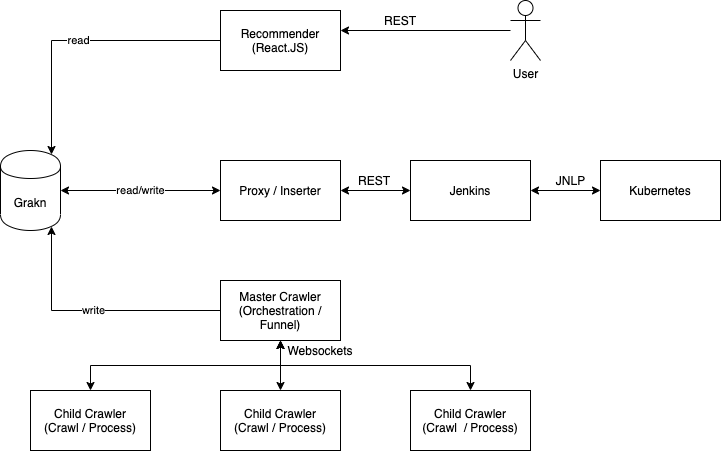
\includegraphics[scale=0.5]{graphics/architecture_v2.png}
    \caption{Architectural representation of the system as a whole}
    \label{fig:architecture}
\end{figure}

\subsection{Database - Grakn.ai}
One of the fundamental decisions is the selection of the database as a lot of other components will have to be built upon it. From the beginning on, it was clear that for building a knowledge graph some sort of graph database could be utilized as it will clearly show the relations of all entities and help in building a recommender system due to the sheer amount of data in the graph.\todo{rewrite}
The implementation could have been done with a NoSQL or a classical SQL database as well, but would have required more linking of data to represent the same sort of result using a graph database.

The first candidate for a graph database that comes to mind is neo4j\footnote{https://neo4j.com}, which is one of the older ones publicly released in 2007\todo{quote https://neo4j.com/developer/graph-database/\#neo4j-overview}. While neo4j could have been used for the implementation, it felt quite outdated when it came to the data representation and their query language "Cypher". Therefore, the graph database Grakn\footnote{https://grakn.ai} was used, which was released in 2016\todo{quote source }.

Grakn describes itself as a knowledge graph engine for the purpose of organizing complex networks of data and making them queryable by performing knowledge engineering\todo{quote https://grakn.ai/grakn-core}. It fully supports the Entity-Relationship model and comes along with a query language called Graql. 

\todo{Deduplication}
\subsubsection{Entity-Relationship model}
Entity-Relationship models are the de facto standard to represent a schema for a graph database.
\todo{redo er model}
\begin{figure}[H]
    \centering
    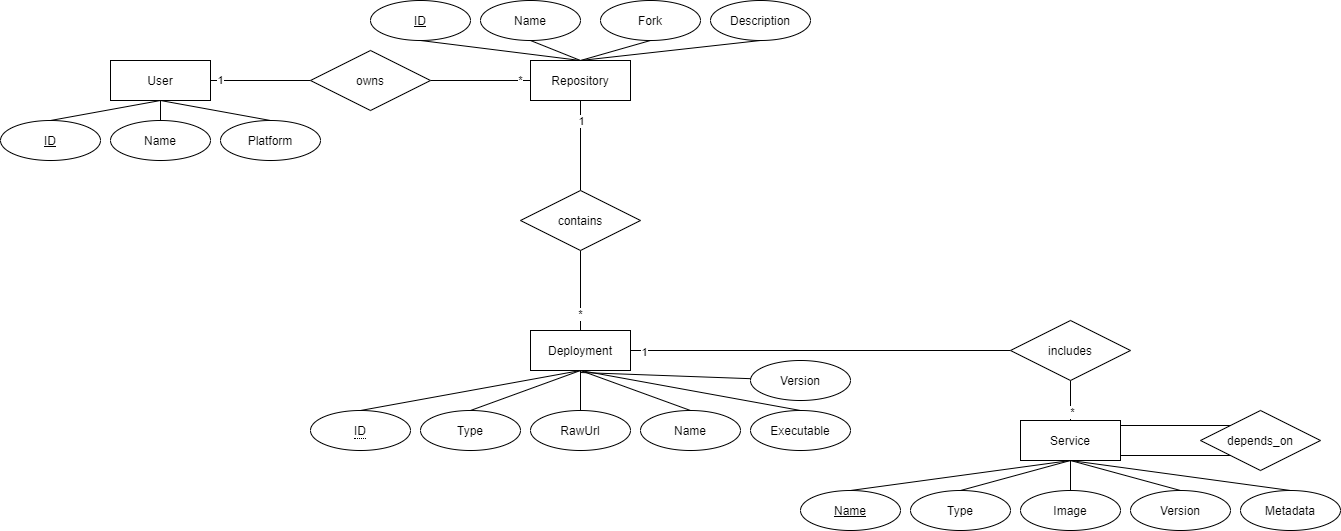
\includegraphics[width=1.2\paperwidth,height=1.2\paperheight,keepaspectratio,angle=270]{graphics/er_database.png}
    \caption{Entity-Relationship model}
    \label{fig:er_model}
\end{figure}

Deployment Scripts do not follow a standard and, therefore, a generalized model has to be created to possibly fit most of them. The focus was lying on the deployment as this entity represents the script itself as a whole. \todo{rewrite} Followed by services that are defined in the deployment script and, therefore, have a direct relationship to the deployment. In a deployment services can occur unlimited times, however, one service can always only have one deployment. This was kept this way as services, depending on the context, can be differently defined in terms of versions or extra attributes. As one is dealing with a graph database, searching for the best possible fits will still work easy as there is a direct relationship between services and their deployment.
Services can as well depend on themselves, meaning that they are more coupled than others, e.g. a database and a backend, for example. Once more this depends highly on the context and will be further explained in another section in this chapter. \todo{e.g. kustomize, kuberentes, helm, docker-compose fit this schema}
As the deployment script is usually embedded in a repository, a coupling is taking place there as well. The repository could represent, in a classical way, a repository on either GitHub or Bitbucket, but could also be a website or documentation depending on where it was found. One repository can hold an unlimited amount of deployment scripts and one can possibly belong to multiple repositories. The simple explanation is that the secure hash algorithm is used as key identification and files that have the same content will, therefore, have relationships added to those repositories as well, while still keeping only one deployment entity in the database. The last entity in the schema is a user that owns unlimited repositories, while one repository can only belong to one user.

One of the favorable aspects of Grakn is how it handles duplicates. As long as one defines unique keys in the attributes of an entity, there will not be a duplicate since those will automatically be dropped on insertion. This will keep the database free from duplicates and allows one to concentrate on the actual implementation of their use case.

The schema is kept general in regards to the domain of different kinds of deployment scripts, while overall favouring the origin from code repositories. A visualization of the schema can be seen in figure \ref{fig:er_model} and gives a self explanatory overview according to current standards in ER models.\todo{rewrite, remove explanaotory overview}

Grakn supports the feature of having an attribute as a key attribute and, therefore, provides uniqueness across one entity based on this key. While Grakn provides its own internal ID, it was useful and necessary to give each entity and relation a self defined key attribute to prevent additional mapping of Grakn ID to e.g. GitHub IDs or other elements in order to uniquely identify one relation or entity.

\subsubsection{Open Source Contributions}
Grakn is a comparatively new graph database which causes its community to still be rather small. Accordingly, problems that have been solved for other graph databases have yet to be covered for this one. Therefore, some contributions to the project around Grakn and its tools have been covered in the implementation of this thesis.

First of all, Grakn comes along with a tool called "workbase", which essentially is an editor to show and edit the graph that the database contains. This is sufficient for most projects where the graph is rather small. The "workbase" is a Vue/React application wrapped in electron, which is a framework to create desktop applications from JavaScript. Therefore, electron is wrapping the files with chromium and node.js to display the application cross platform. The "workbase" comes along with some flaws as graphs with nodes and edges in the 100.000 area will crash the application due to the limited amount of memory assigned to the chromium process. Even in the area of 10.000 and more, the application starts to stutter under the heavy load.

Therefore, the first contribution in the domain of Grakn is a converter from Grakn to the the Graph Exchange XML Format (GEXF), which is essentially a file format to describe complex networks structures.
The advantage of GEXF is that it is an open specification and, therefore, implemented and used by a variation of applications and tools. One of these tools is Gephi - the open graph viz platform that allows to visualize and analyse networks of sizes in the area of multiple million nodes and edges. Another tool is the NetworkX\footnote{https://networkx.org/} framework for python, which allows to load and write GEXF files and , therefore, analyse networks further in the python universe.

The Grakn to GEXF converter reads a provided Grakn schema and generates proper queries for each entity and relation, followed by querying the database for the results and writing the results to a valid GEXF file. This, in return, can be further used by the tools mentioned earlier. Overall, this will help to further analyse the graph as Grakn itself does not provide any tools for layouting, clustering coefficient, community detection and other metrics that might be interesting to extract out of a graph.

Another open source contribution was done in the direction of cloud compatibility as the open source version of the database does not come along with e.g. a helm chart or, in general, kubernetes manifests to deploy and seed a database one has to build the compatibility themselves. It is important to note that the Grakn database is split between a server and a console (cli) component, which are bundled into one docker image. While this makes it easier to e.g. debug the database it is not suitable to run as a sidecar container, as one simply does not need the server component and even then one might run into the problem of seeding the database \todo{rewrite}. The database can only be seeded if it is running, which makes kubernetes init containers useless as those will run before the actual container is running. Therefore, a sidecar is needed, meaning an additional container in the same pod to seed the database as soon as the server container is up and running. While this sounds relatively easy, the Grakn console nor the server provide a health point to check whether the database is really running. Yes, one can probe the port of the database but this will not guarantee that the database is really ready to receive connections. Therefore, the second contribution is a sidecar container, containing a slim alpine image with the Grakn console and a startup script to check for the database for receiving connections and, if needed, seed the database with a schema that can be mounted into the container.
One of the important points of infrastructure as a code is reproducibility, meaning if one runs the code on different systems it should still result in the same end product, thus a manual seeding of the database would not be suitable.

\subsection{Distributed Crawler}
First and foremost, the main part of the implementation is the so-called "distributed crawler", which follows the master and node pattern, where one entity is the master that controls the spawned nodes. In this thesis, it can also be seen as an orchestrator/information funnel and the crawling/processing unit. The reason for calling it a distributed crawler is that the overall function of this implementation can be seen as a crawler and distributed in the sense that the nodes can be distributed across multiple data centers or even be used on edge nodes with the appropriate implementation.\todo{rewrite}

The implementation was done using Node.js, which is an asynchronous JavaScript runtime that allows to run JavaScript outside of the browser and potentially build scalable applications. One of the big advantages of Node.js is that one can use the synergies of running JavaScript on the server-side and client-side. While this might not be the first thing that comes to mind when thinking about a distributed crawler, it does come in handy as a lot of services offer an API\footnote{Application Programming Interface} that returns JSON\footnote{JavaScript Object Notation} objects. These JSON objects are easier to manage in their native environment compared to other programming languages, where one would rely on a third party implementation and a lot of serialization as the implementation was simply not meant for that environment.
As JavaScript runs in a JavaScript engine, the V8 engine developed by Google, it can be extended by creating C++ modules to make certain functions quicker as those would natively run on the system.

The master and crawler nodes are all based on one unified code base. The only difference between the two is the addition of the database connection and the orchestration routes which are both parts of the master node. The default startup parameter for a node is to act as a crawler and connect to the master, which can be changed by setting one environment variable called "TYPE" to "master". The node would, therefore, load the database module, orchestration routes and use the master implementation of the communication channel instead of the crawler one.
The benefits of a unified code base are that the application could be extended in the future in order to support e.g. leader election or let the master act as a crawler as well. Depending on the processing power provided, the master could handle, on top of its own capabilities, the ones of a crawler as well and, therefore, provide more coverage of crawled sources.
Leader election, shortly explained, is that e.g. 4 spawned crawler would elect one of their own to be the master node, which often works based on either "first come first serve" basis or other defined constraints.

On a fundamental level, master and node are web servers providing a REST\footnote{Representational State Transfer} API, that allows one to trigger functions either from outside or from the application itself. REST comes along with well-defined methods using "GET", "POST", "DELETE", "PATCH", and some others. In the context of the distributed crawler, the most used methods are "GET" and "POST", as one either wants to receive information or in a sense add information, while "POST" is often used to as well incorporate functions that are not covered by the other methods.
While a REST API grants a good interface for a user or another application, it is not very well suited for bidirectional real-time communication. As the crawlers are potentially distributed over various data-centers, it can be difficult to keep track of every single one of them, especially for the master as one would need e.g. a domain or another unique identifier to connect to all nodes prior to deploying the master. To counter this issue, another communication channel was introduced - the so-called WebSockets - which allows a real-time bidirectional communication where only the crawler would need to know the unique identifier of the master, instead of the other way around. WebSockets, initially originating from the web browser domain to allow client-server communication, can also be used as a pure client-server communication without a web browser due to Node.js . WebSockets use a TCP socket to communicate through and are on the same OSI layer as HTTP and make use of channels that client and server have to subscribe to, to be able to send and receive messages about a specific topic.\todo{rewrite} This bidirectional communication channel will be part of further subsections.

\subsubsection{Information funnel}
One of the functions of the master node is to act as an information funnel or a proxy to the database. This makes the implementation of the crawler nodes easier as one does not have to worry about connecting to the database and can just use the bidirectional communication channel with the master. From a security point of view, it might also be easier to keep only one communication channel secure compared to multiple small ones, depending on the setup of multiple locations.

Crawlers are essentially preparing and processing what they have crawled completely on their side and send the finished result to the master, which in return inserts the results into the database. The established bidirectional communication channel will be used, keeping additional overhead small compared to other ways of implementing it.\todo{rewrite}

\subsubsection{Orchestration}
As the master and node pattern already suggests, controlling is one of the aspects of a master node. In this case, the job orchestration will be handled from the master node. Therefore, the master provides a REST API that can be consumed by e.g. a user or some sort of automation like cron jobs that trigger crawling on a weekly basis. This could have been implemented using WebSockets as well, but a REST API is easier to consume compared to establishing a socket connection and then sending a message for a specific topic.

While orchestration is a REST API route, it utilizes the WebSocket to send messages to its connected nodes and uses those as well for calculating windows that have to be crawled. A window, in this sense, is a range where the crawling should start and end (more details on the exact reasoning will be covered in the subsection on crawling). The orchestrator has a minimum and maximum value in between which should be crawled, which then in return is divided by the amount of crawlers that are available at the point of receiving the request for orchestration. Each crawler, therefore, receives a window that should be covered.

\subsubsection{Crawling}
The implementation of the crawler makes use of the strategy pattern, which is a behavioral software pattern that allows selecting a strategy/implementation during runtime. This means in particular that there is a generic interface with the defined functions that have to be implemented by each strategy. In Node.js there is no classical object orientation that a lot of people might know from Java. Therefore the implementation makes use of a class that implements the generic interface that then each strategy can extend and implement. Further on there is one main class, which initializes the required strategy during runtime by making use of a simple switch case.

While this gives one a lot of flexibility and options to further extend this with other strategies it also brings along a couple of negative aspects like having to know which strategies are available and some extra effort into handling the implementation.

The first data source to be crawled and therefore the first strategy was for GitHub. GitHub is the biggest collection of public repositories and therefore offers a good starting point to cover roughly over a million deployment scripts in the case of docker-compose.
GitHub offers an API already in its third iteration with various REST endpoints that return JSON. These can be used for crawling GitHub, which can be done in various ways depending on the information that is required. In case of deployment scripts one would be interested in repositories that house those scripts.
One way to tackle this issue is using a breadth-first search algorithm that traverses through users and their repositories and continues by traversing through their contributors and their respective repositories. Random users could be retrieved by utilizing the GitHub api and the contents of a repository could be analysed by cloning the repository and running a quick find script for a selected deployment script as those usually have a similar naming scheme for the same type of tool. Looking at GitHub as a network graph, this strategy might not find all users that have deployment scripts as not all users have to be connected through one way or another. On top of that one spends a lot of time traversing through users and repositories that are not anyhow related to the topic as in the end deployment scripts are compared to e.g. programming languages etc. a niche topic.

Another way to approach this topic is to utilize a GitHub api that allows one to search through the code of all public repositories and therefore be more precise as it will directly return users and repositories related to the topic. This provides the starting point for the GitHub crawler strategy. As GitHub is quite popular and offers its API for free some of those API routes come with limitations, especially in something so resource-intensive as searching code through all public repositories.
Therefore the first limitation that GitHub introduced for the "search REST endpoint" is that only authorized users can use this function and with that, the second limitation comes along that requests will be limited to 30 per minute. To circumvent those two limitations each crawler gets assigned a designated GitHub Account with username and token to authenticate against the API and in case of running into the 30 requests per minute limit the crawler will sleep in intervals till the limit is lifted again.
The next limitation is that GitHub will only return a maximum of 1000 results per search query. While this seems difficult to bypass, GitHub brings along the proper tools to do so. One of the query parameters of the "GET" request is simply called "q" and allows one to build complex individual queries that are unique in itself and therefore offer up to 1000 results per query. The query parameter "q" can be extended to include the file name and file extension. Deployment scripts are often written in YAML\footnote{YAML Ain't Markup Language} and have come along with the extension ending "yaml" and "yml". Therefore doubles the number of search results in the case of YAML specific deployment scripts as one can vary between those two different spellings. The most important factor for circumventing the limit of 1000 results is to utilize the size of a file. GitHub allows one to define the size of a file, that you are searching for, in bytes or in a byte range, meaning one could search for all files in a range of 100-102 bytes or simple in the use case of the thesis to search per byte. This would allow one to create for the same file a unique query every single time.
Of course, GitHub has a limitation for this one as well and only allows to find files up to 384 Kilobyte, which in the context of this thesis is negligible as deployment scripts rarely touch the two-digit Kilobyte area.

Theoretically speaking 384 million files could be covered by just utilizing the size factor without even utilizing such things as extensions, order, or sorting. With those included depending on the type of deployment script, one could easily cover up to a billion search results.

To summarize the GitHub API, it comes along with a lot of limitations but at the same time with all tools needed to circumvent those limitations and therefore covering almost all public repositories.

This should give one a perspective as well on why one would utilize a distributed crawler as this allows to cover a much wider area much quicker by spawning more nodes. As previously mentioned in the part about orchestration a window area is defined for crawling, this is limited from 50 bytes to 384 Kilobytes as a 50 byte deployment script will most likely just include the very basics of its potential. One crawler does not cover the full range, except its the only crawler available, but rather the window that was set by the master node.

\subsubsection{Processing}
Processing was built similar to crawling, meaning it is based on a strategy pattern to be as flexible as possible and gives a certain extensibility for future projects. As it is based on the strategy pattern it comes along with the same advantages and disadvantages as already described in the section about the crawling.
While the crawling itself only covers the points of collecting data, the processing step is the predecessor to inserting the data into the database, but therefore the collected data has to be first brought into alignment with the database schema, earlier described in the section about Grakn.

For this the processing step fetches the deployment script or uses an already provided script and parses the script with a yaml parser, as most deployment scripts are defined in this structure, and creates arrays of entities and relations necessary to satisfy the database schema. This yaml parser will automatically discard all deployment scripts that could not be parsed as those would also not be able to be parsed by the final product, e.g. docker-compose. Therefore all data in the database are syntactically correct and can be further used by e.g. docker-compose or depending on the strategy the tool that was kept in mind for it.

In the case of docker-compose, the script will be parsed and split into the entities of services and deployment. For relations it will be parsed into includes and depends\_on, where includes is the general relation between service and deployment and depends\_on describes the possible dependency of a service to another service, e.g. dependency of database and application.

After completely processing the deployment script and general information about the origin the processed data is sent to the server component or informational tunnel using the bidirectional channel of the WebSocket.

\subsubsection{Data insertion}
After successfully collecting and processing the data the last step is to insert the data into the database. For this step, each entity and relation has its own template, which in the end results in one query for inserting the selected type. This template system is built on a similar thought as the strategy patterns, as a template simply resembles a strategy for a certain provided type. The information funnel, therefore, iterates through each array and selects the proper type to then insert the data.
Grakn is built in a way to first create a database connection, followed by a session, followed by a transaction for either reading or writing and as the last step one has to close the transaction again to commit the actual data or to properly close the reading.
Each connection will use a certain amount of memory to keep the connection alive and each insertion will come along with a certain amount of processing power as everything has to be linked in the graph.
The writing transaction can contain an unlimited amount of queries to insert, but one has to be careful as duplicates will cause this write transaction to fail as a whole, meaning that data that might be unknown will not be written to the actual database. Therefore for this implementation, each query was treated as a single write transaction to circumvent possible data loss. This was done as a user can have an unlimited amount of repositories and therefore possibly deployments or a deployment is used by different users in different repositories and thereby still having a commonly known entity. It is important to collect as much data as possible as deployments that are contained in multiple repositories might be of greater importance than deployment scripts that are unique, but this will be covered in the evaluation chapter.

The initial database connection and session creation don't have a time constraint or are important for actual data commitment, but in case of failure, a new session will be created as it can't be verified that the current session is still valid.

\subsection{Distributed Analysis}
To further analyse the data a system was required that could potentially deal with a lot of data but at the same time not interfere with any running processes. A distributed system that could scale horizontally similar to the concept of the crawler could further complement the whole system. This once more would be a microservice itself and decoupled from the rest of the architecture, meaning possible flexibility in the choice of tooling and implementation. Therefore this section will deal with the choice of tooling, different possible tools, vulnerability scanning, calculation of a score that will further on be used for the recommendation system, and isolation.

\subsubsection{Choice of Tooling}
To determine the final choice of tooling for the task of a distributed analysis one has to consider what has to be achieved, how flexible it is, and whether it can be extended in the future. Time is not too much of importance in this part as due to possible horizontal scaling this can be complemented by simply running it on more hardware.

The task that had to be solved was to run a rather linear task of executing the deployment script, and thereby determining whether the deployment script is executable or not, followed by a vulnerability scan to determine a security factor, checking the deployment script for best practices and in the end doing some later on explained calculations and sending the results back to an API that updates the database with those results.

The first iteration brought forward a couple of possible candidates. One of those is the possibility of using a Continuous Integration (CI) system, which is known for running a lot of tests parallel, which can, depending on the CI, be extended with the usage of plugins and therefore is quite flexible and extendable. Another option was to simply create a REST API that runs certain predefined steps on the provided data. The last option was to use a workflow engine, which is more known in the area of business processes, but in the end, all of it is a rather linear process, which could also be done by such an engine.

All of those options bring along some positive and negative aspects and all of them would be capable of further analysing the data and calculating a score based on the flow earlier described.

Starting off with the option of creating a REST API and processor for doing those simple steps. While this gives one a lot of flexibility and expandability, it will at some point run into the problem of properly isolating the process that is executed by running the deployment script. As this thesis mainly focuses on the aspects of docker images, which are in itself already an isolation, it will at some point encounter problems with possible port mappings from local ports to remote ports or mounting and using of the same files or folders. To fix this issue one could wrap the REST API into a docker container itself and run it in Kubernetes, while this would diminish the issues it would arise new ones. Suddenly routing would become a problem as one would have to spawn a new endpoint for each analysis one wants to run, which in return would mean that either another component is necessary to make sure that only one REST API receives one data package and therefore having another master - node pattern.
Therefore this option was dismissed as the problem has been solved by a lot of other people already in the form of either a workflow engine or a CI system.

Using a workflow engine would already solve the problem of running a certain process in order, but at the same time introduce new issues as workflow engines, in general, come along with an extra component that monitors and manages the processes, hence the engine. They are not made to transport a lot of data between workers and thereby require an extra database to partly save data in the database to transfer information from one worker to another. For the concept of isolation, a workflow engine would exist and have workers spawned that all deal with certain steps, but this does introduce another problem at the same time as one might not know prior how many workers of each task type are needed as some tasks are quicker than others and also introduce the overhead of having to clean up the workspace to have a neutral ground for each task execution. While a workflow engine is certainly an option to solve this task the lack of proper scaling and the additional need to keep the workspace clean dismissed this option as well.

The last option was to use a continuous integration tool, which exists in a broad spectrum from SaaS (Software as a Service) tools to self-hosted tools, from open source editions to enterprise editions. In the end, most of the currently existing CI tools solve the same problem in a similar fashion. The option of using SaaS was not really possible as the tool would not be used in the way it was intended to be used, as unknown code should be covered where the test has to be as general as possible and SaaS tools usually require one to create a file or reference in the code repository of a project to confirm actual ownership of the code and at the same time provide the tasks or tests that should be run for common testing.
For the purpose of the thesis, Jenkins was used, which described itself as an open-source automation server\todo{insert https://jenkins.io reference} and is often used in the area of continuous integration and continuous delivery. It is known for being extendable due to the sheer amount of plugins that exist for it as its first stable release was in 2010. Jenkins is essentially a CI/CD tool, but at the same time can be extended and run any process that one would want to run and thereby was from a technical point of view a good choice for this project.

\todo{e.g. Jenkins + Kubernetes, conftest}
\subsubsection{Importance of Isolation}
To further explain the choice of Jenkins one has to think about isolation. The payload that is being executed is unknown as the deployment script was written by a third party. If talking about e.g. docker-compose the damage that can be done by executing it is rather slim as one would have to break out of the container itself, but as the project can be extended by other possible candidates it's good to find a solution that fits possible future extensions as well. On the other hand, docker-compose can build local images as well that could possibly copy files from the system and later on use them in a malicious way by uploading them to an attacker's storage. Therefore it is important to use an extra layer of isolation.

Jenkins, with the use of plugins, supports a multitude of options of where to actually run the pipeline.
Possible options are to execute those pipelines on the Jenkins instance itself, which if it is hosted in the right environment could be enough already, but at the same time, it would contradict the requirement of scaling it horizontally as the instance would be limited be the resources it is assigned to or the resources of where it's running. While it's possible to have multiple Jenkins instances running and control them with a proxy in front of it to route traffic to A or B depending on the workload of one instance, it is not a best practice and rarely seen in an actual working environment.

Another way to achieve isolation and horizontal scaling is to deploy so-called Jenkins agents to dedicated machines with the sole purpose of executing Jobs, which in the sense of Jenkins is the execution of a pipeline. While this is a better option than executing pipelines directly on the master instance it still comes along with limitations as one needs to set up the agents manually and configure them to talk to the master instance. For the communication, there are different protocols that can be used, which are WebSockets, JNLP, or the usage of Kafka via a plugin. WebSockets are still in beta stage\footnote{https://github.com/jenkinsci/remoting/blob/master/docs/protocols.md} and not widely used same as the Kafka plugin, which is not in beta anymore but simply not as widespread as JNLP. JNLP is the Java Web Start protocol and makes use of a TCP connection in the end.

Coming to the cloud era tools like Docker and Kubernetes gained a lot of traction and while Jenkins was built in an era prior to that the possibility of plugins enables Jenkins to fully exhaust the possibilities of the cloud.
Mounting the Docker socket directly into Jenkins, which enables Jenkins to directly talk to Docker and run pipeline steps in a predefined container is one possibility, but limits Jenkins to the local resources and is not compatible with scalability and proper isolation as the Docker socket is shared and containers binding to local ports would possibly break it for other running pipelines. To stay within Docker one could utilize Docker Swarm to spawn agents that communicate back to the main Jenkins using the JNLP protocol. While this is a valid option it comes with some limitations as it overcomplicates the pipeline due to the requirement of starting each extra required tool manually using "docker start" and "docker exec" to interact with it.

Kubernetes on the other hand provides proper isolation and allows to scale horizontally only limited to the number of nodes provided. The concept of pods allows the structuring of pipelines in an easier way compared to Docker Swarm. A pod is a collection of containers that all share network and storage, which in the context of Kubernetes make it easier to interact with. E.g. a pod has a Docker in Docker container to provide a Docker socket to run e.g. docker-compose files, a container running the vulnerability scan tool, and another container running ubuntu or alpine for additional tooling. In the end, the pod always houses a JNLP inbound agent as well to create the connection to the Jenkins master. Compared to Docker Swarm one does not have to start each required container individually but all of them are started and ready to use from the beginning of the pipeline and the shared network and storage make it easier to interact with files and services from different containers whenever needed.
Further on to complement Jenkins the option of Kubernetes was used to use a cluster to house all running pipelines.

\todo{possible limitations of Kubernetes?}
\subsubsection{Vulnerability Scanning}
To define a score it might be of interest how vulnerable a docker image is. A docker image is essentially a snapshot of a subset of an operating system, meaning that any vulnerability that wasn't fixed at this point in time will still exist in the image till it's rebuilt without the usage of a cache as often Docker just reuses layers if not otherwise instructed. The same can be said for any programming language running inside it e.g. Java, NodeJS, ...

For this purpose one can make use of vulnerability scanning tools, where currently three popular options exist, those being Anchore Engine, Clair, and Trivy.
All of them solve the issue of scanning images in different ways, all of them utilize a database filled with vulnerabilities called CVE (Common Vulnerabilities and Exposures). CVE is a standardized list of vulnerabilities, which makes exchanging and reporting them easier.
In the end, all three scanners have different accuracies for detecting vulnerabilities with no clear winner when comparing them using the same images. See figure \ref{fig:docker_comparison} for comparison.

\todo{add source https://www.a10o.net/devsecops/docker-image-security-static-analysis-tool-comparison-anchore-engine-vs-clair-vs-trivy/}
\begin{figure}[H]
    \centering
    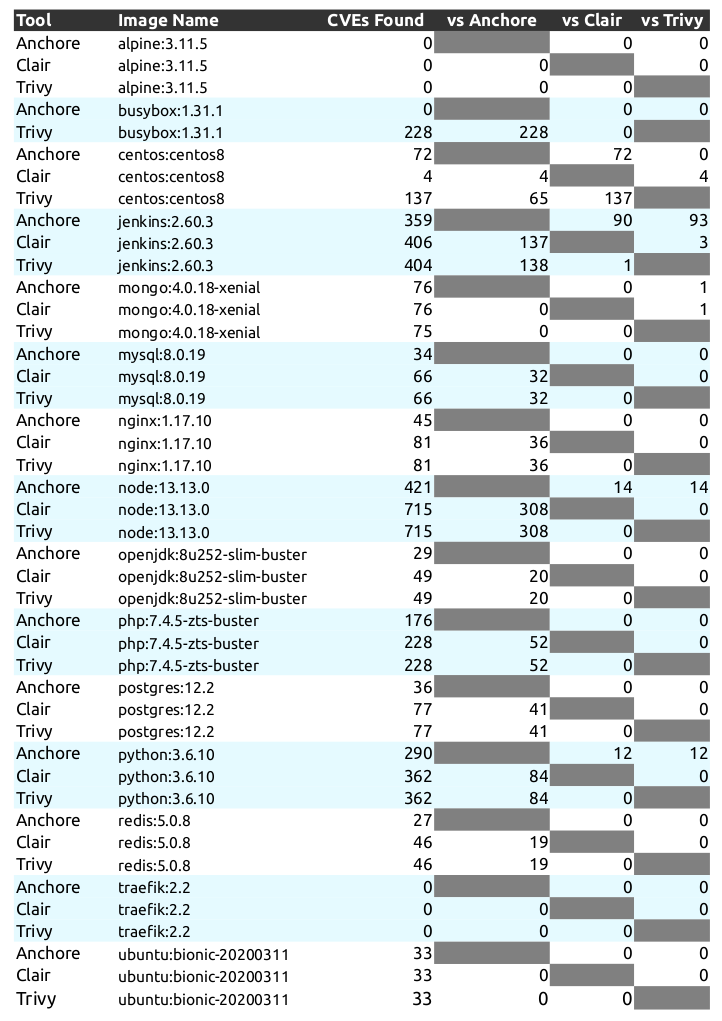
\includegraphics[scale=0.5]{graphics/Docker-Image-Static-Analysis-Tool-Comparison-Table.png}
    \caption{Comparison of Anchore Engine, Clair, and Trivy}
    \label{fig:docker_comparison}
\end{figure}

Some of the tools are easier to implement than others for the purpose of e.g. continuous integration, which is more or less the case for this thesis. Anchore Engine and Clair have to be deployed as a service and need to be accessible for the pipeline. In the case of Kubernetes, this isn't an issue, but it comes along with additional overhead as those tools were simply not developed as a target of CI. Anchore Engine in this case is better than Clair as it comes along with a ready to use CLI, while Clair requires one to use a third party implementation to interact with it. Trivy was built for the purpose of CI and can be integrated as another container in the Kubernetes pod, which then pulls the latest database filled with CVEs and runs the scan against the defined images in the pipeline, e.g. locally built images or images pulled from Docker registries.

Trivy was selected due to its easier implementation and amount of output it delivers when detecting vulnerabilities, as those can be further used for calculating a score. First of all, it delivers IDs, names, and descriptions of a vulnerability and more important the severity, which is categorized in critical, high, medium, low, and unknown. While this is already a good indication of how severe a vulnerability is, Trivy delivers additional metrics as well according to the "Common Vulnerability Scoring System" (CVSS), which is an industry-standard for scoring vulnerabilities. The CVSS is divided into three metric groups, which are base, temporal, and environmental, each consisting of further metrics to determine a final score for each group \todo{reference https://www.first.org/cvss/v3.1/specification-document}.
From those metrics, some interesting metrics are e.g. the Attack Vector (AV), which describes how possible the exploitation of a vulnerability is, or the User Interaction (UI), whether another user is required besides the attacker for the exploitation to succeed. Besides that, there are many more metrics that are evaluated to determine a final score and can be read up in the official specification provided by the FIRST.Org, which houses the CVSS special interest group that is already working on the next version of the specification.
Finally, the CVSS score is divided into numerical ranges to determine the severity, which can be seen in table \ref{cvss_table}.
\begin{table}[h!]
    \centering
    \begin{tabular}{ |c|c| }
    \hline
    Severity & Base Score Range \\
    \hline
         None & 0.0 \\
         Low & 0.1-3.9\\
         Medium & 4.0-6.9\\
         High & 7.0-8.9\\
         Critical & 9.0 - 10.0\\
    \hline
    \end{tabular}
    \caption{CVSS v3.0 Ratings}
    \label{cvss_table}
\end{table}

As the CVSS is an open specification it can be used by anyone and different organizations have the goal of providing a database with a CVSS score for each identified vulnerability. These organizations are in particular Red Hat and the National Institute of Standards and Technology (NIST). Metrics from both databases can differ as metrics within those metrics can be evaluated differently by different organizations, therefore for the consistency of this thesis the database of the NIST was chosen due to the overall amount of rated vulnerabilities compared to Red Hat.
\subsubsection{Calculation of Score}
For the calculation of a score, one has to take a look at all the steps that would be executed by the pipeline. Some of those steps were already described in detail e.g. vulnerability scanning but others like best practices or execution of the deployment script were only briefly mentioned.

The execution of the deployment script shall determine whether the script can be run at all or not, this metric shall help how useful the script might be for usage as a non-executable script might need extra data or images, which are not accessible to the public and thereby of less interest to one. For this, the Docker socket, in the Kubernetes pod of the agent, is directly used to execute the script and afterwards check all containers whether they are either running or exited with a code other than successful. Either result will be set as an environment variable in the pipeline and used later on.

Next on the file length is determined as the longer the file the more the file might be of interest to a reader as it contains more information compared to a basic default script.

For determining whether best practices were followed a tool called Conftest is used, which is published by the Open Policy Agent project under the hood of the Cloud Native Computing Foundation. Conftest enables developers to simply test their structured configuration data \todo{reference https://github.com/open-policy-agent/conftest }, which YAML is considered as well.
These best practices are opinionated best practices defined by the author and kept general as docker-compose in itself is kept simple. Following best practices are checked for in case of docker-compose: \\
\begin{itemize}
    \item images should be pinned, meaning the latest tag should not be used
    \item images should have a tag as otherwise latest is used implicitly
    \item the compose file should state a version
    \item a build should state an image, which docker automatically uses for tagging
    \item dependencies should be set if a database is involved
    \item if a network is defined then the global networks should be set as well
    \item if a volume is defined then the global volumes should be set as well
\end{itemize}

Conftest checks against these predefined rules and returns the number of tests failed and passed, which can be further used to extract a numerical value.

The step of vulnerabilities scans was already covered in detail, but there is a difference between scripts that were executable and those not. The following is another point why Trivy was used as it allows to scan local images and remote images. In the case of non-executable scripts, the images used are being parsed from the script and then analysed by Trivy as those images will likely not exist in the local context. For scripts that are executable, the image is derived from the list of all containers that are either running or have run, this covers all locally build images as well. Those are saved locally through docker as an archive and can be further analysed by Trivy. This would not be possible in the case of Clair or Anchore Engine as the actual analysis is run remotely.

As the last step, the score is calculated by using normalization. Each of the previous steps resulted in a numerical value one way or another. Four values exist of different importance. Thereby both the vulnerability score and the best practices score are given a 1/3 of the total score. It is important to know whether a file is executable or not, but at the same time, the script still brings valuable information and is thereby given 1/6 of the total score. The file length is given a 1/6 as well as the longer the better but at the same time there is a limit of a maximum of 300 lines as anything above this value is most likely not bringing any value as said before docker-compose is a rather simple system that does not have too much complexity to justify such a long file.
All values were normalized in the range of 0 to 10 and afterwards scaled according to their percentage of the total score. For this, the min-max normalization was used as all of the values had predefined lower and upper limit. While a Z-score normalization would be preferable there was no historic data that could have been utilized.
\todo{this could be something that could be done in the future based on the current data}

Other values that were considered that could be tested for but left out were startup time and choice of the docker registry.
The startup time was not a metric that could be anyhow justified to be free of interference. There are a lot of factors that can change this value even if the same script is run multiple times. E.g. current workload of the node that the pod is running on and thereby possibly less available resources compared to a previous run. One may argue that resource limits should be set for the Jenkins agents, but as the payload that is running is completely unknown at startup time it could possibly interfere with the successful execution of some scripts. On top of that a network interference can happen as well in case a container is pulled slower from the registry or the building of an image takes longer due to a low download speed. Thereby the time it takes to execute a script was left out as a lot of factors play into it.

The choice of registry was an acceptable point till the introduction of vulnerability scans as a step into the pipeline as some registries scan their pushed images by default for vulnerabilities. This registry, in particular, is Quay\footnote{https://quay.io}, but at the same time, Docker's own registry and Google offer this service as well if enabled. Thereby all registries are considered equal in the sense of feature parity. Overall there has been quite a shift in the area of Docker registries recently, but this will be covered further in the evaluation. \todo{Dockers monetization strategy and amazons newly announced registry} \todo{possible last time that something like this can happen as docker will soon switch over to deleting old images that are not used anymore}

Overall the score is a numerical value between 0 and 100 and can further on be used for the recommender system.

\subsubsection{Orchestrator / Funnel}
Similar to the already described orchestrator and information funnel in the distributed crawler, a control unit was needed as well for the distributed analysis to orchestrate new jobs for Jenkins and update the database with the scores returned from those jobs. This orchestrator consists of a simply REST API, an inserter, and a queue.

The REST API consists of two routes. One has the purpose of updating the entry in the database with the new values in case of a successful run and the other one has the purpose of removing failed builds from the queue to free it up for new job runs.

The queue is a simple singleton that keeps track of two arrays for database entries that need to be processed and entries that are currently being processed. Its main functions are to return a random object from the to be processed queue and to keep this exact queue free from duplicates as the database will return the same objects for the same query and thereby duplicates are removed at the application level.

For orchestrating new jobs the inserter will run certain functions based on a temporal value. Every 30 seconds the database will be queried for yet unprocessed entries till it houses a predefined maximum value of 100 entries. Every 2 seconds the length of the process queue is checked and depending on a predefined value a REST request is sent to Jenkins to schedule a new job with the required parameters to run the job. This predefined value is set to 20 and can be changed depending on the setup as it highly depends on the Kubernetes cluster. For the purpose of this thesis, it was set to 20 as it seemed the most stable in the provided environment.

The orchestrator acts as a proxy between Jenkins and the database for reasons of reliability and abstraction purposes.
An implementation could have been done without the necessity of an additional proxy by extending the Jenkins pipelines with two simple steps. The first step would utilize an additional container with e.g. Node.js to run the Grakn.ai library to query for database entries. This would be followed by the steps explained earlier in the part about the calculation of the score and finished by another step to update the values in the database for the previously queried entry. This would likely be not as efficient due to querying the database for a single entry, which would result in the same entry for each pipeline till the entry is updated with new values, thereby running the pipeline 20 times at the same time would result in 20 pipelines running the tests for the same values. The reason being that the database simply caches queries that are not unique for quicker responses. Therefore a proxy was implemented to take care of scheduling jobs, updating the database and keeping duplicates out of the system. Being its own microservice the implementation could have been done in any language but was done with similar frameworks as the information funnel.
\subsection{Frontend}
For the graphical user interface of the recommender system, the language of JavaScript and its frameworks were used once more. While everything is a microservice in itself already and thereby decoupled from the other services, the implementation can be done in any language, but the synergies of using the same language for everything were used due to the prior knowledge and background in the Node.js framework.
The frontend could have been written in pure JavaScript, HTML, and CSS, but for the purpose of this thesis, a frontend framework was utilized. It gives one a certain abstraction compared to doing everything in its pure form and allows one to write everything in JavaScript. There are plenty of frontend frameworks to choose of with similar popularity and use cases, in the end, it comes down to preference as the job could be done in any of those. Due to prior knowledge in this topic, there were two candidates to choose from, which are React and Vue.js.

React was developed in 2013 by Facebook and offers a modular system, meaning one develops modules that bundle logic and presentation in one object. This allows the exchange of those modules across different projects and rapidly increases the development of new applications as a lot of problems have already been solved and published by someone else.

Vue.js was developed in 2014 and published by Evan You. In its scope, it's the same as React and only differs in nuances like easier to master, but lacks in regards to publicly available modules. In comparison, the community of React is much bigger and therefore provides more modules even for topics that are niche and thereby have a small community in the first place. The difference of the community size and thereby popularity can simply be explained by having such a big company like Facebook as a project maintainer.

Due to the support of some niche modules, the framework of React was selected.

While React is a framework itself a lot of frameworks building up on React have emerged that all deal with different problems. React in itself is a pure frontend framework and has thereby no out of the box support for a backend, which is still needed to interact with the database and deliver the initial application. Thereby the Next.js framework was selected as it complements React by offering a simple out of the box solution for creating a simple API.

The recommender system offers an input field to type in the image or images one is looking for and a drop-down menu that offers all available types of deployment scripts. The inputs are sent to the recommendation API, which in return queries the database for 10 deployment scripts with the highest score that offer all typed in images if no such script exists then it tries to find deployment scripts for each image individually. The returned entries build a selectable table in the frontend, which if clicked on sends another API request to fetch all services and its connections related to the selected deployment script to in return visualize the deployment script as a graph of all connected services.

Overall the frontend is kept simple to offer the user a self-explanatory user experience and allows to quickly find related deployment scripts that can be used as inspiration for ones own script. Therefore the type of recommender system is a content-based recommender system as all scores are precomputed based on the implementation explained prior.
\section{Expandability}
The focus of the thesis was on deployment scripts related to docker-compose, but one of the aims of this contribution was to implement everything as expandable as possible.
Starting with the database the entity-relationship model was created as generic as possible with options to extend it to a different type of sources and deployment scripts by offering the type parameter, which make it easier to select certain types while querying. On the other hand, the database can be extended as well by creating new keyspaces related to different types of deployment scripts. These could utilize the same schema, but would probably benefit from being decoupled from other deployment scripts in terms of performance as not a single graph with all information has to be kept but rather graphs related to the same type.

During the chapter about the distributed crawler, the strategy pattern was already introduced, which offers the development of strategy in terms of crawling sources and processing.
For crawling it could be extended to different code repositories like Bitbucket, GitLab and privately hosted repositories. On top of that even such things as search engines could be utilized as those crawl most of the internet already and offer indexed lists, which could offer a similar efficiency as the GitHub code API. The search term for all crawling strategies is variable, meaning it can be used for any type of deployment script as long as it has a similar naming scheme e.g. Kustomize in case of Kubernetes. Strategies for other deployment scripts could be developed as well, which don't follow a naming scheme e.g. Helm, which offers a registry for their so-called charts. For something like Ansible it might be a bit more difficult as it doesn't offer a common filename nor a unique identifier in the script, but even for Ansible GitHub offers eighty thousand unique files called "playbook.yml" and custom strategies could be built that utilize other methods to find Ansible scripts. The table \ref{deployment_script_occurrences} shows approximately the amount of related deployment scripts of some tools on GitHub. An exact number can not be given due to the GitHub API experiencing a timeout after a certain time and returning all results it collected till then.

\begin{table}[h!]
    \centering
    \begin{tabular}{ |c|c| }
    \hline
    Type & Occurrences \\
    \hline
         Docker-Compose & > 1.260.580 \\
         Vagrant & > 256.348\\
         Ansible & > 121,388\\
         Kustomize & > 65.481\\
         Helm & 2061*\\
    \hline
    \end{tabular}
    \caption{Approximately found deployment scripts on GitHub. * Helm artifact repository}
    \label{deployment_script_occurrences}
\end{table}

The processing of those deployment scripts supports the strategy pattern as well and a strategy has to be developed for each deployment script that one would want to insert into the database as each type of deployment script is unique and has to be altered to the database scheme.

For the distributed analysis the underlying layer of Jenkins and Kubernetes can be used as well and only a new job has to be developed, which could consist of similar tasks compared to the docker-compose pipeline. The deployment script could be executed in an isolated environment, some best practices could be tested with the help of Conftest, vulnerabilities could be scanned as well for defined images in those deployment scripts and the file size could be utilized as a metric as well. Overall the currently defined pipeline could act as a very good starting point for other types of deployment scripts. In case of Kustomize and Helm, the docker in docker container could be switched for a kubernetes in docker container, which allows testing Kubernetes related scripts in a continuous integration environment.

For the proxy, an additional instance could be spawned that is configured by providing environment variables with all related information to trigger the proper pipeline and query the required entries. It's simpler to spawn an additional proxy compared to making the proxy compatible for multiple types of deployment scripts.

The frontend just requires an additional entry in the drop-down menu to support a different kind of deployment script. The rest should be compatible with the current system.

Looking at it each component from the microservice perspective each implementation could be replaced by another one as long as it follows the predefined interfaces. In the case of the distributed crawler, the master or node could be replaced by another implementation. For the node it could be even contemplated, e.g. have 2 nodes running the initial implementation and another 2 nodes a newer implementation. The same goes for pretty much every implementation except Jenkins as it the replacement for this component would also mean the proxy would need to be adjusted.

In summary, the implementation explained and provided by this thesis can be extended for additional deployment scripts and due to the architectural choice of the microservices can be extended even further by providing own implementations with the same behaviour.

\section{IaC of implementation}
\todo{optional chapter}

%\section{Open Source}
%\subsection{GitHub}

%\section{Architecture}
%\subsection{Microservices}
%\subsection{Software design pattern}
%\todo{Strategy pattern}
%\todo{Singleton}
%\subsection{Node.js}
%\subsection{React}

%\section{Protocols}
%\subsection{WebSocket}
%\subsection{REST}
%\subsection{gRPC}
%\subsection{JNLP}

\chapter{Evaluation}

This chapter is divided into the evaluation of the quantitative metrics captured by the implementation of this thesis and the network analysis of the graph, which can be generated out of the graph database and further analysed.

All previously described implementations were wrapped into individual docker containers, to first and foremost adopt "Infrastructure as Code", but also to use Kubernetes as scaleable infrastructure. The setup was running on a self hosted Kubernetes cluster using 5 baremetal machines, consisting of 2 master nodes and a total of 5 worker nodes, including the master nodes.

The graph database was occupying one of the 5 worker nodes, using a special taint to only schedule the database on this single node. Due to the usage of baremetal servers, and extra schedule taints, the local disk was directly mounted into the container to provide faster throughput compared to using a virtual disk. Each individual server provided 8 cores and 16 Gigabyte of memory. Typical cloud offers from Azure, AWS or GCP were not accessible.

The remaining implementations, e.g. Jenkins, the crawler and the proxy were all scheduled across the remaining 4 nodes.

The byte range of 0 bytes to 384.000 bytes were crawled within two weeks and no additional crawling was done afterwards, meaning the results are purely from one run, which covered all possible bytes that GitHub allows. The analysis took another two weeks and was done after the two weeks of crawling the results to not overload the graph database. The reasoning for this will be explained further down below.

Considering the crawler implementation one can compare the total amount of available "docker-compose" files that the GitHub API provides to the total amount the crawlers have crawled. As already described in the contribution about the crawler \todo{add reference to chapter}, the GitHub API has some limitations that affect the implementation as well. While providing a horizontally scaleable solution, which is only limited by the amount of GitHub tokens supplied, the GitHub API still has some nowhere described complications. This thesis and included test execution were all done under the terms of the GitHub Terms of Services, which states that the crawling of public data is only allowed for scientific works and require the results to be public \todo{quote TOS}. The TOS also states that the usage of the GitHub API is only allowed with a fair usage in mind, meaning one is not allowed to differ too much of the average usage of certain GitHub API routes. Not complying with those rule will likely result in a termination of ones account. During the data collection period, a total of three GitHub accounts were created with the sole purpose of crawling public data, which is only available with a valid GitHub account. Due to the excessive usage of the code search GitHub API route one out of three accounts received a so-called shadow ban. A shadow ban is a system to hide the fact that the user received a temporary termination. A shadow banned user can still use every GitHub API, but the results returned by the API are always empty even though they still conform the expected schema. GitHub as a provider of this free service does not provide any additional documentation about this system. It is not known at which point the account received the shadow ban, but it is to assume that this limitation was applied after the crawling period of two weeks, since the crawler still reported valid results back compared to two weeks later.

Besides this limitation the only other limiting factor was the 16 Gigabyte of memory for a graph database, which turned out to be not an issue by the memory itself, but the graph database had some blocking operations in the write process, which was heavily relied on. In a recent version this issue was fixed. This issue might have had an impact on the total amount of crawled files, since the database started to block any further insertions. To detect those issues a service called Sentry\footnote{https://sentry.io} was used, which sent alerts for not handled issues like the blocking of the database. This might have had an implication on the total amount of crawled files. The community edition of Grakn does not provide any Kubernetes manifests, thereby, manifests and settings have to be created by oneself, which likely results in a not entirely production ready setup, since the production ready setup with multi sharding is only reserved for the commercial usage.

In the following the actual amount of crawled entries will be compared to the possible and total amount of crawled items that the GitHub API returns. Both will be compared to each other by using a column chart.

\begin{figure}[H]
    \centering
    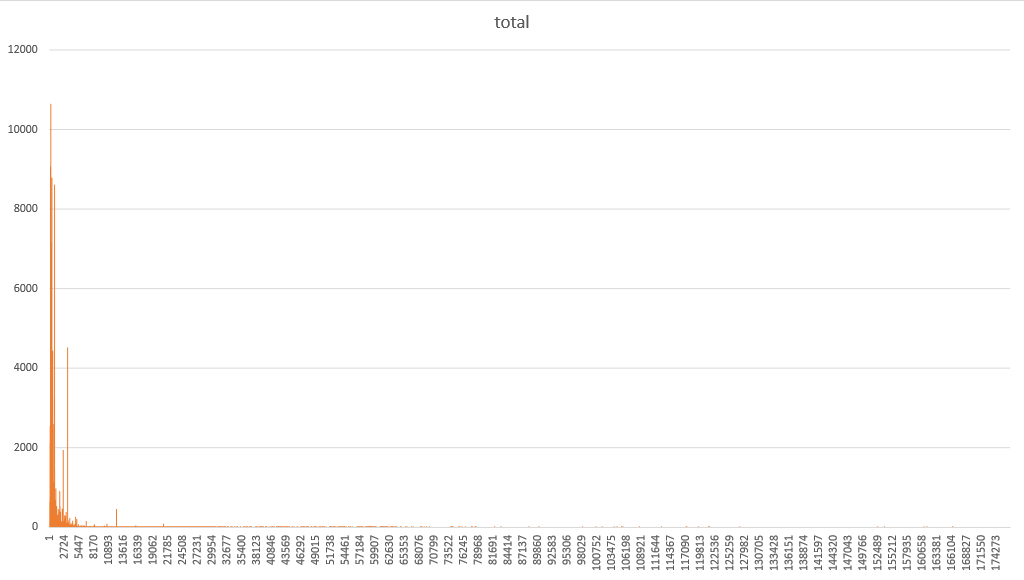
\includegraphics[scale=0.5]{graphics/stats_total.png}
    \caption{Chart representing the total amount of possible results using the GitHub API for the term "docker-compose"}
    \label{fig:stats_total}
\end{figure}

The chart \ref{fig:stats_total} represents the total amount of possible results for the term "docker-compose" using only the GitHub API. The Y-Axis represents the total amount of found occurrences and the X-Axis represents bytes. For this graphical representation the range from 0 to 175.000 was used, since between 175 Kilobyte and 384 Kilobyte are only an additional 200 results. There is a total of 1,1 million results in the chart, most of them clustered around the file size of 100 to 200 bytes, which can be explained due to "docker-compose" files being rather simple and short compared to other deployment scripts. 

\begin{figure}[H]
    \centering
    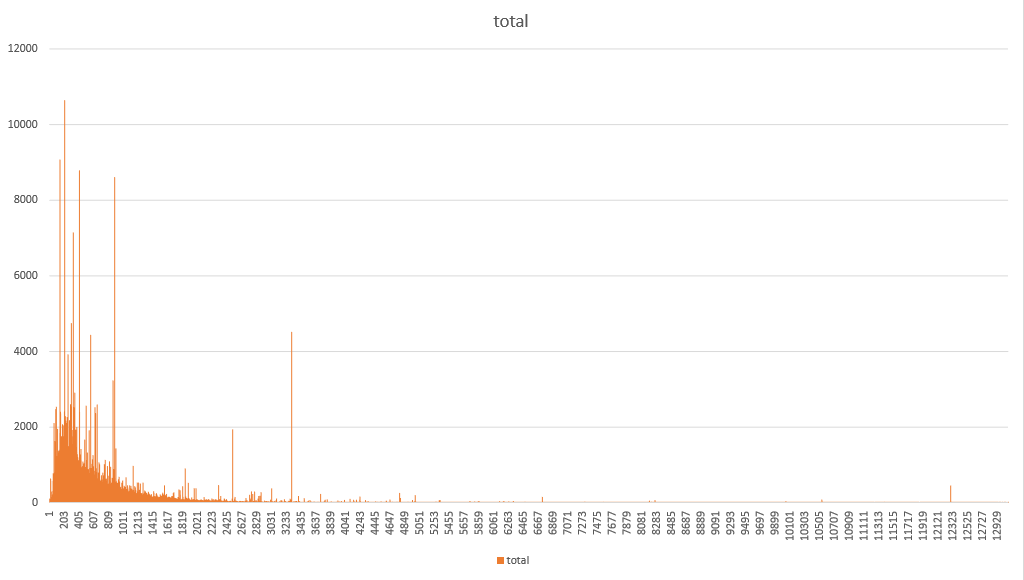
\includegraphics[scale=0.5]{graphics/stats_range.png}
    \caption{Cutout from \ref{fig:stats_total} for the range from 0 to 3000 bytes }
    \label{fig:stats_range}
\end{figure}

The cutout from the range 0 to 3000 bytes as seen in figure \ref{fig:stats_range} shows that the most files are in a range from 100 to 400 bytes and then slowly traverses towards 0, with as seen in figure \ref{fig:stats_total} occasional occurrences in a higher byte range. Both charts \ref{fig:stats_total} and \ref{fig:stats_range} represent the best case if GitHub would return more than a 1000 results for a single query and are both incomplete as well, since GitHub will only return the amount of found results till it receives a timeout. Meaning that running the same query twice would likely result in different results, as the API receives a timeout and returns all found results so far. This behaviour occurs as well when querying single pages, since GitHub only allows a maximal result of 100 entries. This could mean that for running one query on page 10 one could receive a 100 results and for another one close to 0, since the API received a timeout before. In case of this thesis this issue was dismissed, as the author has no influence on the actual implementation of GitHub and it could be mitigated by running the crawling process multiple times for the same bytes.

\begin{figure}[H]
    \centering
    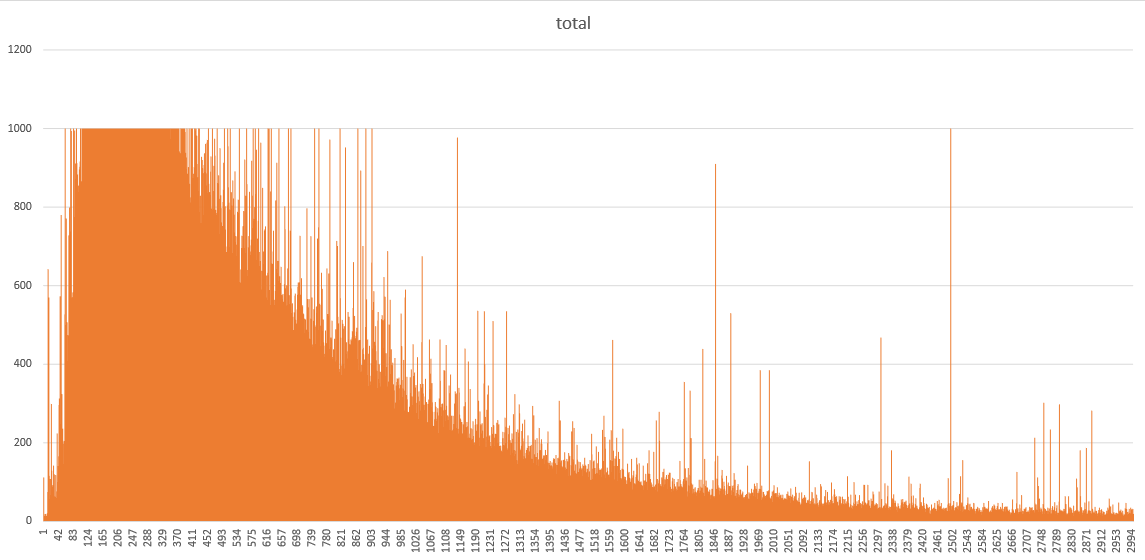
\includegraphics[scale=0.5]{graphics/stats_range_max_possible.png}
    \caption{Cutout from \ref{fig:stats_total} for the range from 0 to 3000 bytes, but a maximum of 1000 results }
    \label{fig:stats_max_possible}
\end{figure}

The chart in figure \ref{fig:stats_max_possible} shall represent the maximum amount of possible results, that can be crawled, since the GitHub API only returns a maximum of 1000 results for a single query. As explained prior for the chart \ref{fig:stats_range}, this does not mean that one will receive a 1000 results, since the GitHub API is nondeterministic.

Further on, the charts for the actual crawled data will be shown, which resulted in 140.000 valid deployments. Valid, since only parseable deployment files were inserted into the database, see \todo{add reference to the explanation in contribution} in the chapter about the implementation.

\begin{figure}[H]
    \centering
    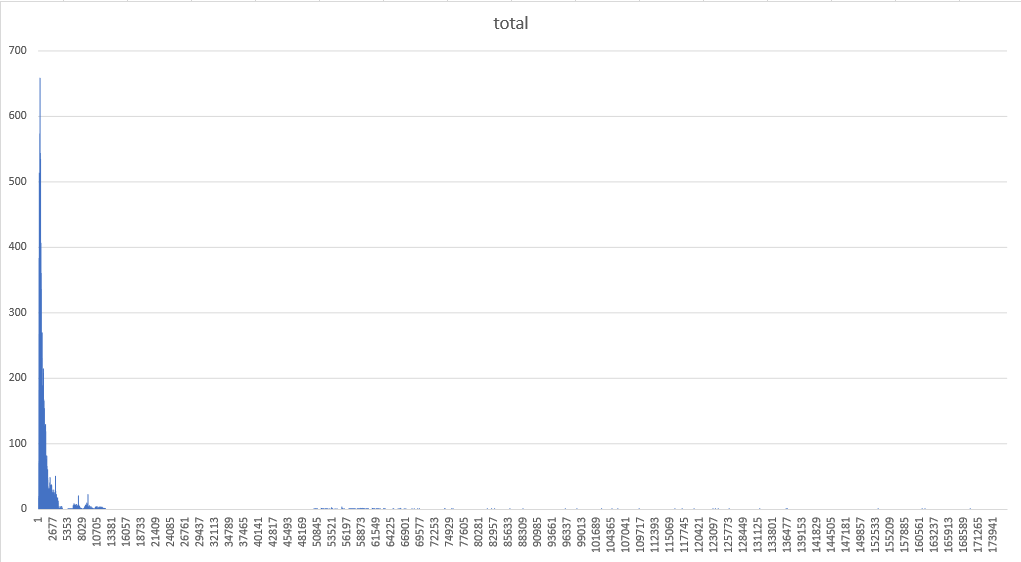
\includegraphics[scale=0.5]{graphics/deployment_stats_total.png}
    \caption{Chart representing the total amount of possible results using the crawler implementation for the term "docker-compose"}
    \label{fig:deployment_total}
\end{figure}

Comparing the figure \ref{fig:stats_total} and the figure \ref{fig:deployment_total}, one may notice a similar representation, which validates the overall implementation, since clusters for similar bytes were successfully crawled with occasional results in the higher byte area.
The chart \ref{fig:deployment_total} also shows that the maximum crawleable number of a 1000 results was never reached, which could be explained by either the nondeterministic behavior of the GitHub API or the blocking process of the database. On the other hand this could simply be explained by non parseable deployment scripts as well, since a lot of people have especially in the lower byte range scripts that are the bare minimum or contain syntactical issues, which cause the parsing to fail and at the same time render the file useless for the "docker-compose" executable as well, since it can not parse the file either.

\begin{figure}[H]
    \centering
    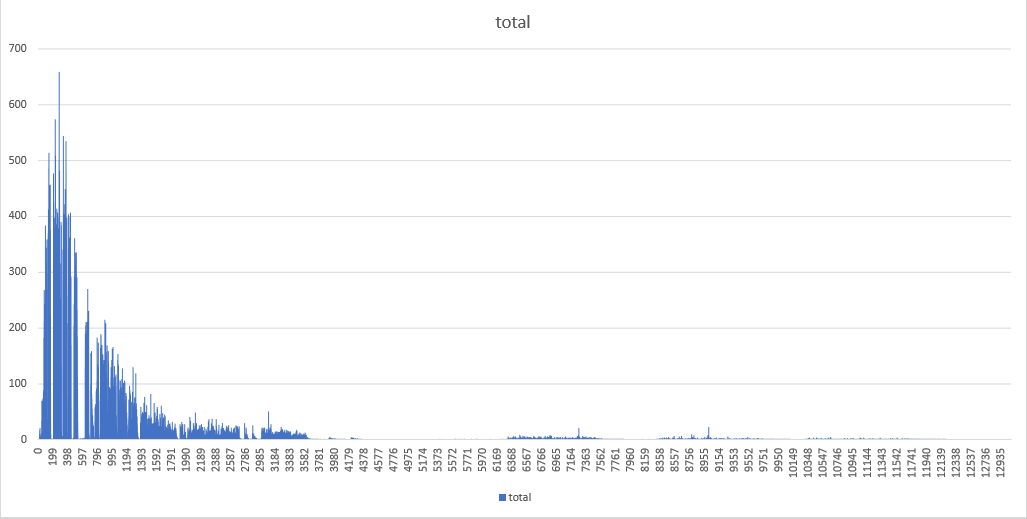
\includegraphics[scale=0.5]{graphics/deployment_stats_range.png}
    \caption{Cutout from \ref{fig:deployment_total} for the range from 0 to 3000 bytes}
    \label{fig:deployment_range}
\end{figure}

The chart \ref{fig:deployment_range} still resembles the chart \ref{fig:stats_range}, but it is visible that that the previously described shadow ban has occurred earlier than expected, since the chart \ref{fig:deployment_range} shows multiple spots where barely any results were returned, e.g. 161-201, 441-481 or 521-641, which mirror the system of a shadow ban. The implementation featured crawler windows, which consisted of a byte range that were individually assigned to each crawler, which in this case could have been assigned to the shadow banned account. During the execution period it was not visible that the account was affected, since it acted as expected and returned results according to the schema.

Overall the GitHub API returned a total amount of 940.000 possible crawleable entries, which can still differ in numbers when actually crawled for due to the way the GitHub API works. A total of 140.000 valid deployment scripts were inserted into the database, which represents 15\% of the total crawleable amount. Limiting factors were in this case the nondeterministic behavior of the GitHub API, the shadow ban system of GitHub and the blocking operations of the graph database. Except the nondeterministic behavior of the GitHub API all other issues can be mitigated for future work, by providing more valid GitHub tokens, which can be switched in case of shadow banned accounts and a more non-blocking graph database. Grakn already provided a patch to resolve the blocking issue, but in the non community edition the graph database can be scaled across multiple Kubernetes nodes as well, since the community edition does not provide any Kubernetes manifests and relied on the implementation of the author.

In total the graph database contains 4,2 million entries, which can be divided into roughly a million nodes, a million edges and two million attributes. Which can be further split down as follows:

\begin{table}[h!]
    \centering
    \begin{tabular}{ |c|c| }
    \hline
    Type & Amount \\
    \hline
         count & 4.279.664 \\
         attributes & 2.546.547 \\
         \hline
         nodes & 836.337 \\
         \hline
         user & 127.084 \\
         repository & 160.506\\
         deployment & 139.469\\
         service & 409.277\\
         \hline
         edges & 896.780 \\
         \hline
         own & 159.834 \\
         contain & 194.797 \\
         include & 404.736 \\
         depend & 137.412 \\
    \hline
    \end{tabular}
    \caption{Graph Database total counts}
    \label{graph_database_total_counts}
\end{table}

The approximately 400.000 services can be analysed further by having a look at the most used images and their versions. This will be divided into multiple tables with different categories, which are databases, programming languages and miscellaneous.

\begin{table}[h!]
    \centering
    \begin{tabular}{ |c|c| }
    \hline
    Image & Amount \\
    \hline
         postgres & 20074 \\
         mysql & 16103 \\
         redis & 13817 \\
         mongo & 11843 \\
         mariadb & 3241 \\
    \hline
    \end{tabular}
    \caption{Top 5 image counts for databases}
    \label{table_image_databases}
\end{table}

\begin{table}[h!]
    \centering
    \begin{tabular}{ |c|c| }
    \hline
    Image & Amount \\
    \hline
         node & 2346 \\
         php & 1121 \\
         golang & 375 \\
         python & 353 \\
         java / openjdk & 325 \\
    \hline
    \end{tabular}
    \caption{Top 5 image counts for programming languages}
    \label{table_image_languages}
\end{table}

\begin{table}[h!]
    \centering
    \begin{tabular}{ |c|c| }
    \hline
    Image & Amount \\
    \hline
         nginx & 8459 \\
         rabbitmq & 3241 \\
         hyperledger/fabric-peer & 2834 \\
         phpmyadmin/phpmyadmin & 2523 \\
         hyperledger/fabric-ca & 2105 \\
    \hline
    \end{tabular}
    \caption{Top 5 image counts for miscellaneous}
    \label{table_image_misc}
\end{table}



Coming to the distributed analysis where Jenkins was used as a base system for running a predefined test for each "docker-compose" file. The tests were conducted for two weeks with a total amount of 60.000 executed tests. By the end a total of 18.000 scripts were successfully evaluated. The failure reasons of the other 42.000 tests can be viewed from different technical perspectives.

For once, public data was crawled and inserted into the database and GitHub repositories were either deleted or made private within this short time period, which accounts to a total of a 1000 repositories. The whole "docker-compose" file could have been saved in the database, but it only has limited further usage, since docker-compose files usually contain a build directive in the file, meaning without the repository the "docker-compose" file can't be executed and this already accounts for a sixth of the score and the vulnerability scan can not be executed in detail as well, which would be worth a third of the whole score. In the beginning, the proxy was missing a denylist causing the 1000 unavailable repositories to be rerun over and over again, but this was fixed during the analysis period.

Kubernetes was used as container orchestration and, as previously described, was set up on dedicated machines, which means the whole maintenance was included as well. A production ready setup was used for the 5 nodes cluster, but after running a total of approximately 20.000 pods no pods and, therefore, no further tests could be scheduled. It turned out that the etcd storage contained too many objects and started blocking the master nodes, which did not respond to any new requests. This caused the whole cluster to stall, since all requests received a timeout. This happened around the 40.000 mark again, resulting in a lot of aborted tests, as a lot of them had stalled.

Overall most of the Jenkins related issues can be mitigated by using managed Kubernetes clusters by e.g. Azure, AWS or GCP with dedicated node pools, which are only used by the CI system.

The score system, explained in the contribution \todo{add reference}, consists of in total 4 different criteria, with each a different significance for the final score. The first third is split into two sixth, since the criteria evaluated in there are of less importance in comparison to the remaining criteria. One sixth considers where a file can be executed or not. Another sixth covers the file length of the file, since the longer the file the more valuable it seems. One third covers the CVSS score, which considers the vulnerability of an image or in this case the vulnerability score of all included images. The last third covers "docker-compose" related best practices.

\begin{figure}[H]
    \centering
    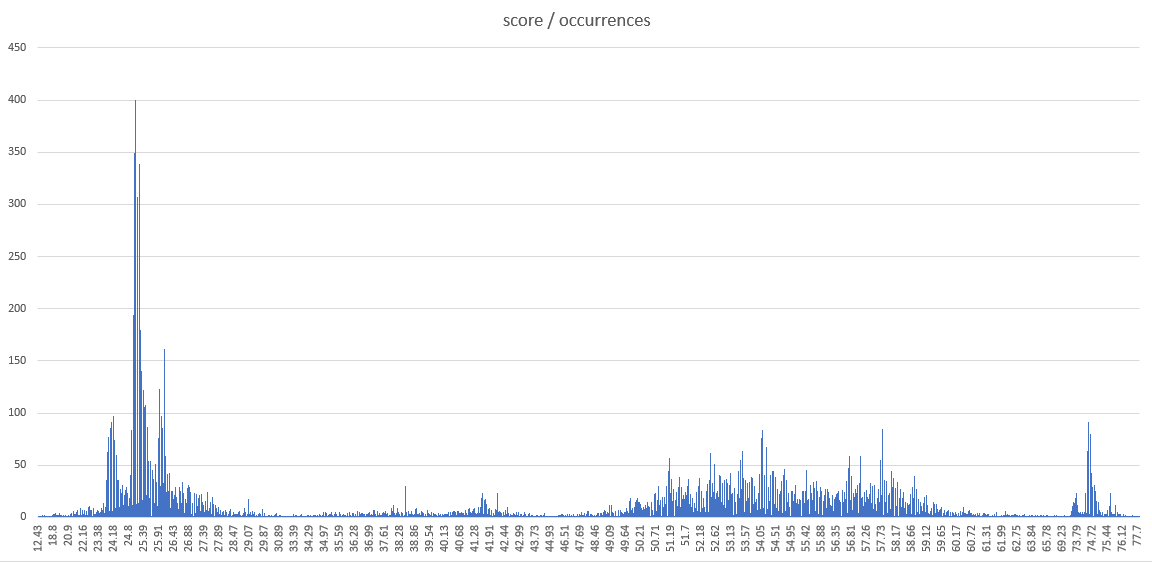
\includegraphics[scale=0.5]{graphics/deployment_score.png}
    \caption{Score distribution}
    \label{fig:deployment_score}
\end{figure}

The figure \ref{fig:deployment_score} shows the score distribution between 0 and 100, where 100 is the best possible score. The X-Axis represents the scores and the Y-Axis are the total amount of occurred scores. The chart shows that there are clusters around the score 24, 54 and 74, which could be explained through the split of the score in four criteria. Some of those criteria are more variable compared to others, e.g. executable is either a true or false and, thereby, contributes either fully or not at all to the score. Taking this fact into account, it's interesting to see that there is no score below twelve, which means that every evaluated deployment script fulfills at least parts of one criteria to the fullest. For the ones around twelve it is to assume that they are executable, since it counts as a sixth of the total score, but at the same time are short and vulnerable. Taking a look at the opposite side of the chart, there is nothing that fulfills a score of a 100, nor is a score close to it. This can be based on the issue of taking the file length too much into account as valuable source, as explained in the contribution part \todo{add reference to part} the file length of 300 as a reference for a "docker-compose" based deployment script might be too much and this unfolds in the chart, since there is a cluster around 74, which will fulfill almost all criteria to the fullest except the file length. For future work this could be changed to the file size, since the file size brings more value compared to the file length. Taking a look at the 180.000 crawled deployment scripts the median of the file length amounts to 22 and even taking the median of the upper part still amounts to 45, meaning that more than 75\% are smaller or equal to the file length of 45. On the other hand taking the file size into account it shows a median of 438 for the 180.000 scripts. This median would have been much more suitable for the score and could be used as a replacement for the file length. Nevertheless, since the file length only accounted for a sixth of the total score and in general has less significance for the value of its content, the score itself and the distribution shown in chart \ref{fig:deployment_score} are still valid and express the importance of the contents of a single deployment script.

\begin{figure}[H]
    \centering
    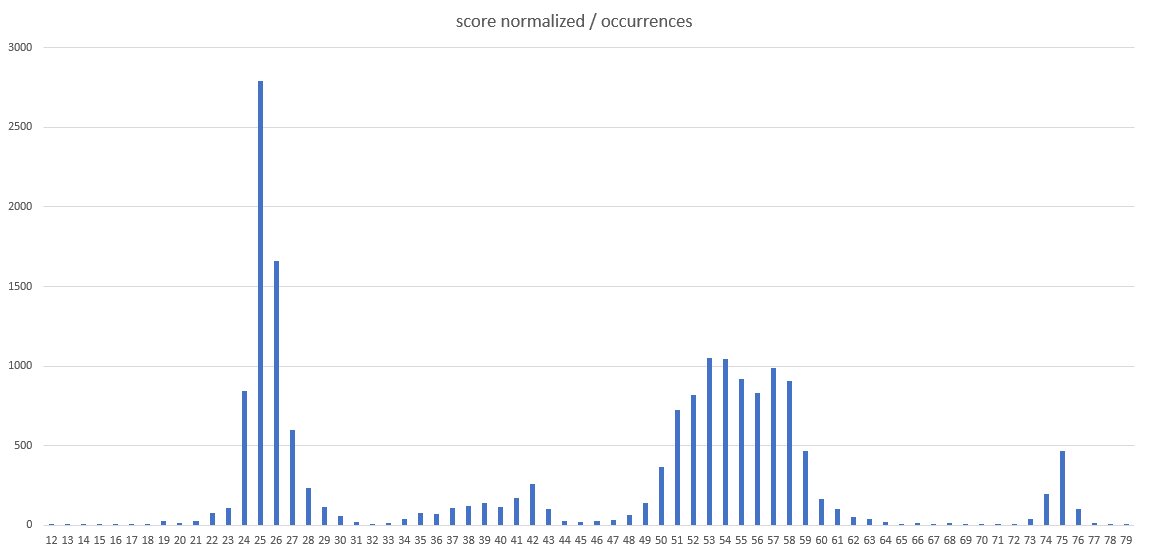
\includegraphics[scale=0.5]{graphics/deployment_score_normalized.png}
    \caption{Score distribution normalized}
    \label{fig:deployment_score_normalized}
\end{figure}

Taking a simplified look at the score distribution in the chart \ref{fig:deployment_score_normalized}, one can see a better picture of the score clusters. For the distribution between the score of 50 and 60 the amount of executable scripts amounts to 99\%, while the total amount of executable files amounts to 56\%. This cluster can be summarized as average but executable, as the deployment script is either fully vulnerable or fully following the best practices or, which is more likely, an average of both criteria.

The CVSS score is the most variable one and looking at the charts of \ref{fig:deployment_score} and \ref{fig:deployment_score_normalized} explain the values inbetween those previously mentioned clusters around the score of 24, 54 and 74.

The score gives an indication whether one script is more valuable compared to another. Still, the suggested scripts should be consumed with caution, since one might not know the contents of one image or the possible dangers of defining specific environment variables without enough care.
For future works the criteria of the file length should be replaced with the file size, as it brings more value compared to the length. The suggestion of using a Z-Score instead of a Min-Max normalization can be dismissed, since the goal of Z-Score normalization is to form the data into a normal distribution, which is not applicable for this type of data. Thereby, the Min-Max normalization is preferred, since the data requires to have the same scale, since one wants to compare across all available data with the same scale.

\begin{table}[h!]
    \centering
    \begin{tabular}{ |c|c|c|c| }
    \hline
    score & image & tag & base image \\
    \hline
         78,69 & linuxserver/letsencrypt & latest & alpine \\
         78,03 & myregistry/simplest-lab & simplestlb, simplestdb, simplestapp & alpine \\
         77,75 & try-webpack & dev & alpine\\
         77,70 & aporeto/apobar & crud & ubuntu \\
         77,53 & python & 3-alpine & alpine\\
         77,53 & traefik & latest & alpine\\
    \hline
    \end{tabular}
    \caption{Images with highest scores}
    \label{images_with_highest_score}
\end{table}

The table \ref{images_with_highest_score} represents the contents of the 5 deployment scripts with the highest score. While the table looks small, some of those images were used multiple times in the same file, making the "docker-compose" files rather complex.
Something that should stick out of the table \ref{images_with_highest_score} is the fact, that most images use alpine as a base image. Alpine compared to other distributions, used for docker, is more secure and simpler, due to the removal of a lot of standard libraries and executables. Due to the removal of such things the resulting image is much smaller and at the same time more secure, since the attack surface is shrinked quite a bit.
The one image that is using Ubuntu in this table is an assumption, since the Dockerfile is not publicly available, nor does the contents of the Docker image give any insights. The image does not contain any executable that one would assume, e.g. ls, echo, cd, shell, bash, and many more. The only thing possible is to gain access to the \$PATH by causing an error, but even this doesn't bring much more information than already known, except for the fact that "snap" is in the path. Snap is a package manager shipped out of the box with newer Ubuntu versions, thereby the assumption of Ubuntu. Nevertheless, this image is much more secure than a default Ubuntu image and shows how to properly secure ones container even against reverse engineering.
Besides alpine as base image, busybox is used quite often as well, since it combines a lot of utilities into a single executable and is perfect for running simple scripts or in the context of Kubernetes as initialization container. Due to its limitied capabilities it's quite secure as well, since there is barely any attack surface.

%Second most important chapter. Verifies the theses defined in the previous chapter. Tries to evaluate and analyze the contribution in qualitative or quantitative terms. Ends with a discussion. Approximately 20 to 30 pages. Can be split into multiple chapters.

% Hier solltest du die limitations deiner Contirbution versuchen zu analysieren. Dies können quantitative sachen sein, wie die limitationen des crawlers wie oft gecrawlet werden kann über github api und wie oft dann andere ergebnisse rauskommen. andere sachen wären zB ob der von dir erstellte score "qualitativ gut" IaC bewerten kann. Für diese unterschiedlichen Punkte sollten folgende Unterpunkte folgen:
%a) Evaluation Setup: hier wird der versuchsaufbau und die durchführung beschrieben. welche größen werden zB gemessen sollte auch beschrieben werden. Womit wird vielleicht das ergebnis verglichen?
%b) Results: Darstellung der Ergebnisse und Beschreibung der Ergebnisse
%c) Discussion: Bewerte die Ergebnisse und ordnete sie ein.
%Am Ende des Kapitels sollte dann eine summary kommen, was der leser gelernt haben soll und welche fragen noch offen geblieben sind für future work und welche forschungsrichtungen man diese arbeit weiter entwickeln kann.

\section{Graph Analysis}
\section{TBD - General Analysis}

\chapter{State of the Art}
\label{sec:stateofart}
The current state of the art can be divided into 4 categories, which are Crawling of Code \ref{sec:coc}, Infrastructure as Code Analysis \ref{sec:iaca}, and Recommender Systems for Developers \ref{sec:rsfd}, and Code Analysis \ref{sec:codeAnalysis}. Those categories are chosen since there is no direct paper related to this thesis, but papers in each of those categories, which are within their categories related to this thesis.
% Related work. Present state of research and applied solutions concerning the different aspects relevant to the thesis. Discuss differences and similarities to other solutions to the given tackled problem. Approximately 10 to 15 pages.

% Länger als Background. State of the Art ~ 4-5 Seiten, aber wichtig Background immer weniger
% (0,5-1 Seite je paper), die sehr ähnlich sind zu deiner Arbeit. Weniger genau Paper, die teilaspekte deiner Arbeit beschreiben (ca. 0,5 Seite je paper). Zusammenfassned dann alle paper die perifär ähnliches beschreiben (typisch sind hier so 4-8 paper pro halbe seite.

\section{Crawling of Code}
\label{sec:coc}
In regards to "Crawling of Code", one of the papers is "Mining the Network of the Programmers: A Data-Driven Analysis of GitHub" \cite{mining} published by Ma et al., which has the goal of collecting public data of GitHub and analysing it as a social network. Within their work, they implemented a distributed crawler, which collected more than 2 million user data from the profile pages on GitHub. Their implementation used a scheduler connected to a MySQL database, which recorded the data, and worker nodes, which used a Breadth-First Search algorithm to crawl the users' profile pages on GitHub by using the follower and followings lists. They applied machine learning to the collected data by selecting certain features like the total amount of stars the user received or the number of repositories the user owns and visualized their findings in charts.
Compared to this thesis they took the approach of a distributed crawler as well since it covers more data more quickly, but they had the advantage of only having to access publicly available data from the GitHub page without having to use their API and its limitations. Due to the usage of MySQL, their findings lack the analysis of social network-related metrics like the average shortest path, the clustering coefficient and its possibility of a small world problem, and many more, which could have been derived by using a graph or graph database. Using a BFS algorithm compared to GitHub API to find possible repositories that own a "docker-compose" file is not feasible, since there are more than 40 million public repositories\cite{githubpublicrepos}, which could potentially contain such files. Crawling each repository would require one to crawl through each possible directory or once more use the GitHub API, this would likely result in an IP address blockage since a GitHub account is not required. In regards to the code collection, this thesis is the most related one in terms of the approach, since a distributed crawler was used.

The paper "Influence analysis of Github repositories" \cite{influencegithub} by Hu et al. deals with the analysis of important and influential GitHub repositories based on publicly available data. Using this data, they created a graph based on the stars a repository received over time by utilizing the GitHub star event. They used several sources to collect this data. One of those sources was the GitHub API to gather metadata on users and repositories. Another source is the "GH Archive"\footnote{https://www.gharchive.org/}, which offers all available event data from 2011 to 2020 and was used as the main driver of their data collection since GitHub itself only offers up to 300 events via their API with a maximum age of 90 days. The setup didn't require any distributed crawler logic, as the "GH Archive" offered all available data without the need to crawl data oneself. In direct comparison, the solution using the "GH Archive" as a data source is a good starting point, but it only offers event data. There is no public repository containing a global index of all available files that are kept in public GitHub repositories. The difference in the approach relies on the usage of a pre-collected data source, which as previously stated is not available for the data, which was required for this thesis. In terms of data storage, a similar approach can be assumed to be used since it was no further described, except for using a database and extracting a graph out of it. While this can be achieved by using a SQL or NoSQL database, the advantages of a graph database overshadow the extra steps required to using a pure SQL or NoSQL database.

A related master thesis "Crawling and Analyzing Repository in GitHub" \cite{Zhang2016CrawlingAA} by Zhongpei Zhang deals with the collection of user and repository data of all repositories with more than 500 stars of GitHub. The goal is to cluster the usage of programming languages according to repositories and users and analyse the data and how programming languages might be coupled together depending on their usage. The thesis does not describe their crawler implementation nor does it describe the database they used, but they describe in detail the process of crawling GitHub, which shows similarities to this thesis in terms of limitations. Zhongpei Zhang heavily relied on the GitHub API in terms of crawling user and repository data, which are both endpoints that allow up to 5,000 queries an hour compared to only 1,800 queries per hour for the code API. Another similarity is the usage of query parameters to create unique queries and receives additional data compared to a standard search.

\section{Infrastructure as Code Analysis}
\label{sec:iaca}
The first paper in regards to the "Infrastructure as Code Analysis" is called "Cloud WorkBench – Infrastructure-as-Code Based Cloud Benchmarking" \cite{cloudworkbench} by Scheuner et al. and describes the creation of a cloud benchmarking Web service with a focus on Infrastructure-as-a-Service clouds. Since cloud benchmarking can be error-prone if done manually, automation was required to verify the validity of the results. For this, the concept of Infrastructure as Code was used, since it verifies that the same resources are created if the same manifest was used and thereby providing reusability and consistency. The software Chef\footnote{https://www.chef.io/} was used as automation and orchestration system to run the benchmarks, which were previously defined in Infrastructure as Code manifests. Comparing this thesis and the paper, it shows similarities in goals and execution since both deal with the benchmarking of a related field in a consistent and automated way. While the paper deals with the benchmarking of cloud providers, this thesis deals with the benchmarking of Infrastructure as Code related deployment scripts. Both projects relied on the concept of Infrastructure as Code since it provides a reusable and consistent way to execute benchmarks with the usage of automation software, which deals with the execution.

The second paper "Testing Idempotence for Infrastructure as Code" \cite{idempotence} by Hummer et al. deals with the testing of the idempotency of Infrastructure as Code scripts with a focus on Chef. For this, a distributed prototype was implemented, which tested 298 so-called cookbooks provided by the Opscode community. Their system consists of a Web interface, which controls the test execution, and various virtual machines, which are each running a test agent. This test agent is an implementation, that executes, intercepts tests, and inserts the results into a MongoDB. The tests itself are run within a Linux container (LXC), which offer proper environment isolation and allow parallel test execution. Overall the idea of this paper goes in a similar direction as this thesis, just with a different goal. Publicly available data was used, while the paper didn't require an additional crawler, due to the manual selection of deployment scripts according to different criteria. Test execution was done in form of a pipeline and proper workload isolation using the most popular tools at that time, which supports the approach in this thesis. While this paper focuses on the idempotence of deployment scripts it does not create a score in any sense, but rather whether a script behaves in the same way if executing multiple times, which could be used as an additional indicator for this thesis in case of the implementation of a Chef strategy.

An analysis of all available non-forked Dockerfiles was done in October 2016 and is described in the paper "An Empirical Analysis of the Docker Container Ecosystem on GitHub" \cite{empirical} by Cito et al. Instead of crawling public data via the GitHub API, a public GitHub archive was used, which is not further described nor properly explained how. The "GH Archive"\footnote{https://www.gharchive.org/} does not contain any data about the contents of a repository, except for event data. To gain additional metadata about the set of 70,197 Dockerfiles the GitHub API was used to be able to connect the information of the Dockerfile better to such things as programming languages or project size. Their goal was to compare the usage of Docker in popular projects to the general GitHub community. A relational database was used as storage. Their implementation involved a Java application, which applied a linter to each Dockerfile and its revisions and inserted the results into the relational database. Manual execution of 560 repositories was done, which resulted in 34\% not being able to build. The lack of version pinning resulted in linting errors for 28.6\% of all Dockerfiles. This analysis was done in 2016 and similar observations can still be done in 2020 in terms of version pinning. The approach was done in a similar way, but with the focus on Dockerfiles instead of "docker-compose" files, while the paper does not try to calculate a score, but rather just express in a binary way, whether a manifest follows certain community-defined best practices or not. Additionally, a distributed system was not used, which could have eased the manual testing and possibly enabled the testing of 70,000 Dockerfiles. Therefore, the paper solely focuses on an overall analysis of all available Dockerfiles on GitHub, while this thesis focuses on deployment scripts and recommending those according to a calculated score. Ideas of this paper, like linting Dockerfiles, could be included in the future work or utilizing the same system to create strategies to execute all 70,000 Dockerfiles in a consistent way.

There is no known paper that deals with the scoring of Infrastructure as Code related manifests. All of the papers presented deal with one aspect in particular, which could in return be used as an indicator of how good a deployment script is in terms of a final score. Overall the presented papers show similar approaches in terms of workload isolation and automation since those attributes are required to verify consistent results.

\section{Recommender Systems for Developers}
\label{sec:rsfd}
"Knowledge-aware Recommender System for Software Development" \cite{Nguyen2018KnowledgeawareRS} is a paper written by Nguyen et al. and proposes a recommender system with a focus on open-source software by utilizing a knowledge graph. This system shall help developers to find similar projects with the same focus or suggesting libraries that similar projects have used. In total, they implemented all known types of a recommender system, each for a different use case. Similar approaches were taken in regards to the knowledge graph, but besides that, the use cases are not comparable since the paper focuses on Maven\footnote{https://maven.org}, an artifact repository.

The paper "A Declarative Recommender System for Cloud Infrastructure Services Selection" \cite{costcalculatorcloud} by Zhang et al. defines a recommender system for Infrastructure as a Service provider. Its recommendation is based on the cost calculation of user-defined services, which those available providers offer. The system shall help a user to decide which provider to select depending on the use case they have. Their implementation consisted of a Web service using JavaScript frameworks as frontend and Java as backend utilizing a MySQL database. The recommender system can be described as a knowledge recommendation, similar to this thesis since it relies on user-defined input to be able to recommend data. Since the data does not resemble a possible social network, nor have any important relations, a relational database was sufficient. A data crawler was not required as well since the data has to be manually collected from the cloud providers public documentation. A score calculation does not take place, since the Web service will return the cost calculations for all cloud providers and a user has to decide and compare themselves between those. A knowledge-based recommendation was used as it relies on user-defined data, similar to this thesis, but has a shortage in actually recommending a final item since all options are presented to the user, which still require the user to review all items to determine themselves the best candidate.

\section{Code Analysis}
\label{sec:codeAnalysis}
Code analysis, in particular static code analysis, is a useful method to assure a certain code quality or find errors before even running a program. While this thesis does not analyse source code of programming languages, it does still statically analyse the deployment scripts for best practices and prior to this even for compatibility of the file schema.
"Empirical Analysis of Static Code Metrics for Predicting Risk Scores in Android Applications" \cite{androidAlenezi} by Alenezi and Almomani conducted an empirical study on the impact of static code metrics and their relation to security vulnerabilities in Android applications. They analysed 1407 pre-selected Android applications by statically analysing the code using Sonarqube and used Androrisk to receive a risk score using fuzzy logic. Furthermore, they categorized the risk scores into No, Low, Medium, and High for an easier prediction model. By using the Spearman's Rank Correlation Coefficient they showed a direct correlation of static code violations to a higher risk score and used this combined with machine learning to classify other applications as well based on this data set. Taking this direct correlation into account it can be observed in deployment scripts as well, since the 5 deployment scripts with the highest score, as seen in Table \ref{images_with_highest_score}, were the ones with the least amount of vulnerabilities and following the best practices, which were derived by applying a static code analysis. To conclude a clearer picture an empirical analysis would need to be carried out on the existing crawled data, but the subset presented in Table \ref{images_with_highest_score} does lead to this assumption.




\chapter{Conclusion}

One page. What have we learned in/through this thesis?

Expected thesis length: 90 pages (+-10\%)

%\chapter{Notes}

Just a collection of random notes about possible findings/decisions. Will later be converted into actual content.

\section{GitHub Crawling}

Different approaches:\\
web ui vs api\\
The web ui is built on the api and can be used with the same query parameters as the api. On top of that the web ui has the same limitations as the api, except possible rate-limiting. Further on the api will be used as it allows to query quicker and with less overhead.\\

directly search for filename\\
search for filename in the description or readme of any repository\\

current limitations:\\
Per search query a maximum result of 1000 entries can be returned.\\
Meaning a naive search for docker-compose would result in a total\_count of 800k results of which you can only view 1000.\\

Ways to mitigate that:\\
GitHub offers various kinds of query parameters\\
<<possible list some and explain>>\\
Querying the api allows only the following parameters, where q is further divided into extra "parameters":\\
q=\{extension\\
file size\\
path\\
file name\}\\
sort\\
order\\
page\\
\\
to get unique urls and to be able to search for more than just 1000 files, we will utilize the size parameter, which allows values of either Integer or Integer..Integer, meaning a range. The values supplied will be interpreted by GitHub as bytes. Therefore we can search for more files as on a byte level files are more likely to be distributed as not all share the same size due to obvious reasons (content). <<refer to how docker-compose files are structured>>

\section{Database}
The aim is to build a knowledge graph or graph in general to be able to utilize it further for either recommender systems or proper analysis of relations between the usage of images.

Comparisson between possible Databases?\\

Neo4j\\
- proper Graph Database\\
- querying feels super outdated\\
- only directed edges\\
- node.js support\\

Grakn.ai\\
- underlying system is a Graph, but more knowledge orientated\\
- designed for machines (output/input)\\
- hypergraph\\
- node.js support\\
\\
Currently in favour of grakn.\\
Next step: define Modell\\
\subsection{Entity–relationship model}
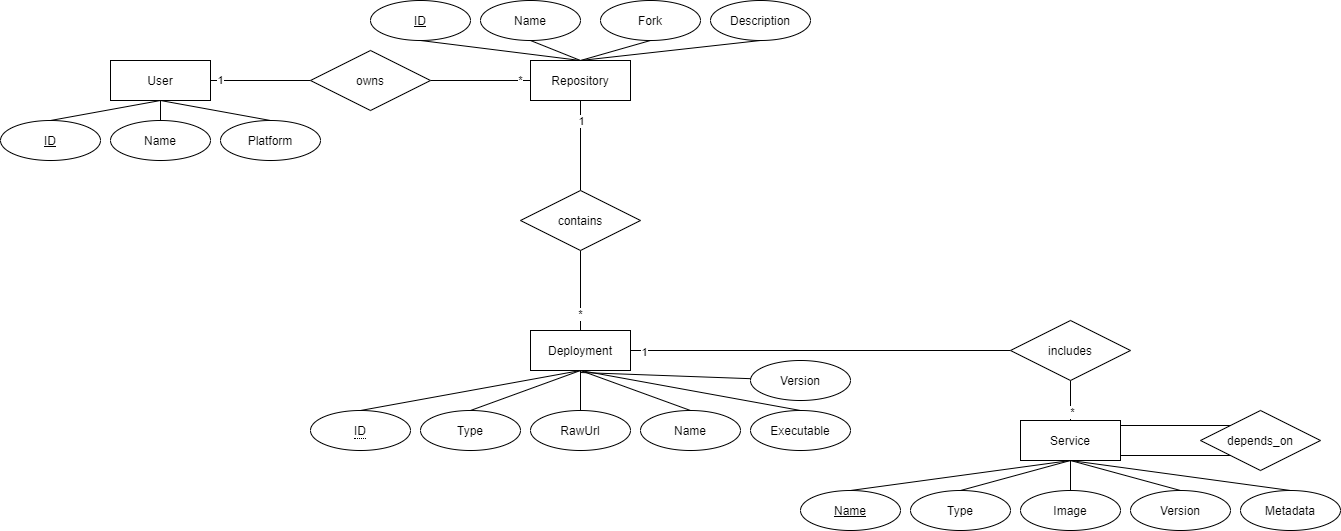
\includegraphics[width=1.2\paperwidth,height=1.2\paperheight,keepaspectratio,angle=270]{graphics/er_database.png}

\newpage
\smallerBegin
\pagenumbering{roman}
\bibliographystyle{plain}

\bibliography{all_publications}

\smallerEnd

%% end of document

\end{document}